\chapter{Propensity Score Matching}

\section{Observational studies}
\noindent {\bfseries Outline}:\\
1. Randomized trial.\\
2. The difference between randomized trials and observational studies.
\begin{itemize}
	\item[$\blacksquare$] Classic confounding setting.
	\item[$\blacksquare$] Ignorability assumption.
	\item[$\blacksquare$] Causal graphs of two situations.
	\item[$\blacksquare$] Good properties in randomized trials.
	\item[$\blacksquare$] Why not always randomize?
\end{itemize}

\noindent 3. How to control for confounding?

Matching. {\color{orange}The basic idea} is to control for confounding, and making the observational studies be likely to the randomized trials.

\noindent 4. Advantage of Matching.

\subsection{Randomized trials}
\paragraph{In a randomized trial, treatment is randomly assigned.} 在随机实验中,每个subject的处理都是随机分配的. 因此处理A的分配与covariates X是无关的,可以移除DAG中X到A的边. 

\subsection{Randomized trail and obsevational studies}
The difference between randomized trail and obsevational studies is shown in Fig.\ref{rmtrail}.
\begin{figure}[htbp]
	\setlength{\abovecaptionskip}{0pt}     %调整图片标题与图距离
	\setlength{\belowcaptionskip}{10pt}
	\vspace{-0cm}  %调整图片与上文的垂直距离
	\setlength{\abovecaptionskip}{-0cm}   %调整图片标题与图距离
	\setlength{\belowcaptionskip}{-0cm}   %调整图片标题与下文距离
	\centering
	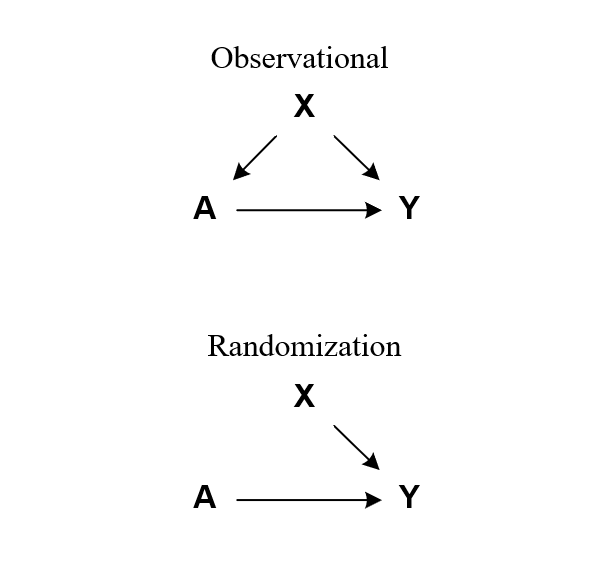
\includegraphics[width=0.6\textwidth]{figure/rmtrail.png}
	\caption{Randomized trail}
	\label{rmtrail}
\end{figure}

在Randomized trail中不存在backdoor path from A to Y. 但是在observation中仍然存在. 我们想要做的就是令observation接近于randomization,消除X对A的影响.

\paragraph{Randomization的作用: }通过随机化分配A,消除X对A的影响.
\paragraph{Good property in randomized trial.}The distribution of pre-treatment variables X will be the same in both treatment groups. e.g. {\color{red} Covariate balance.}

\paragraph{Balance is the distribution of these covariates to be the same in two treatment groups.}因此,如果两个treatment groups的outcome不同,不会是因为两组X的不同所导致的,而只能是处理的不同导致的. 

\subsection{Why not always randomize?}
\begin{figure}[htbp]
	\setlength{\abovecaptionskip}{0pt}     %调整图片标题与图距离
	\setlength{\belowcaptionskip}{10pt}
	\vspace{-0cm}  %调整图片与上文的垂直距离
	\setlength{\abovecaptionskip}{-0cm}   %调整图片标题与图距离
	\setlength{\belowcaptionskip}{-0cm}   %调整图片标题与下文距离
	\centering
	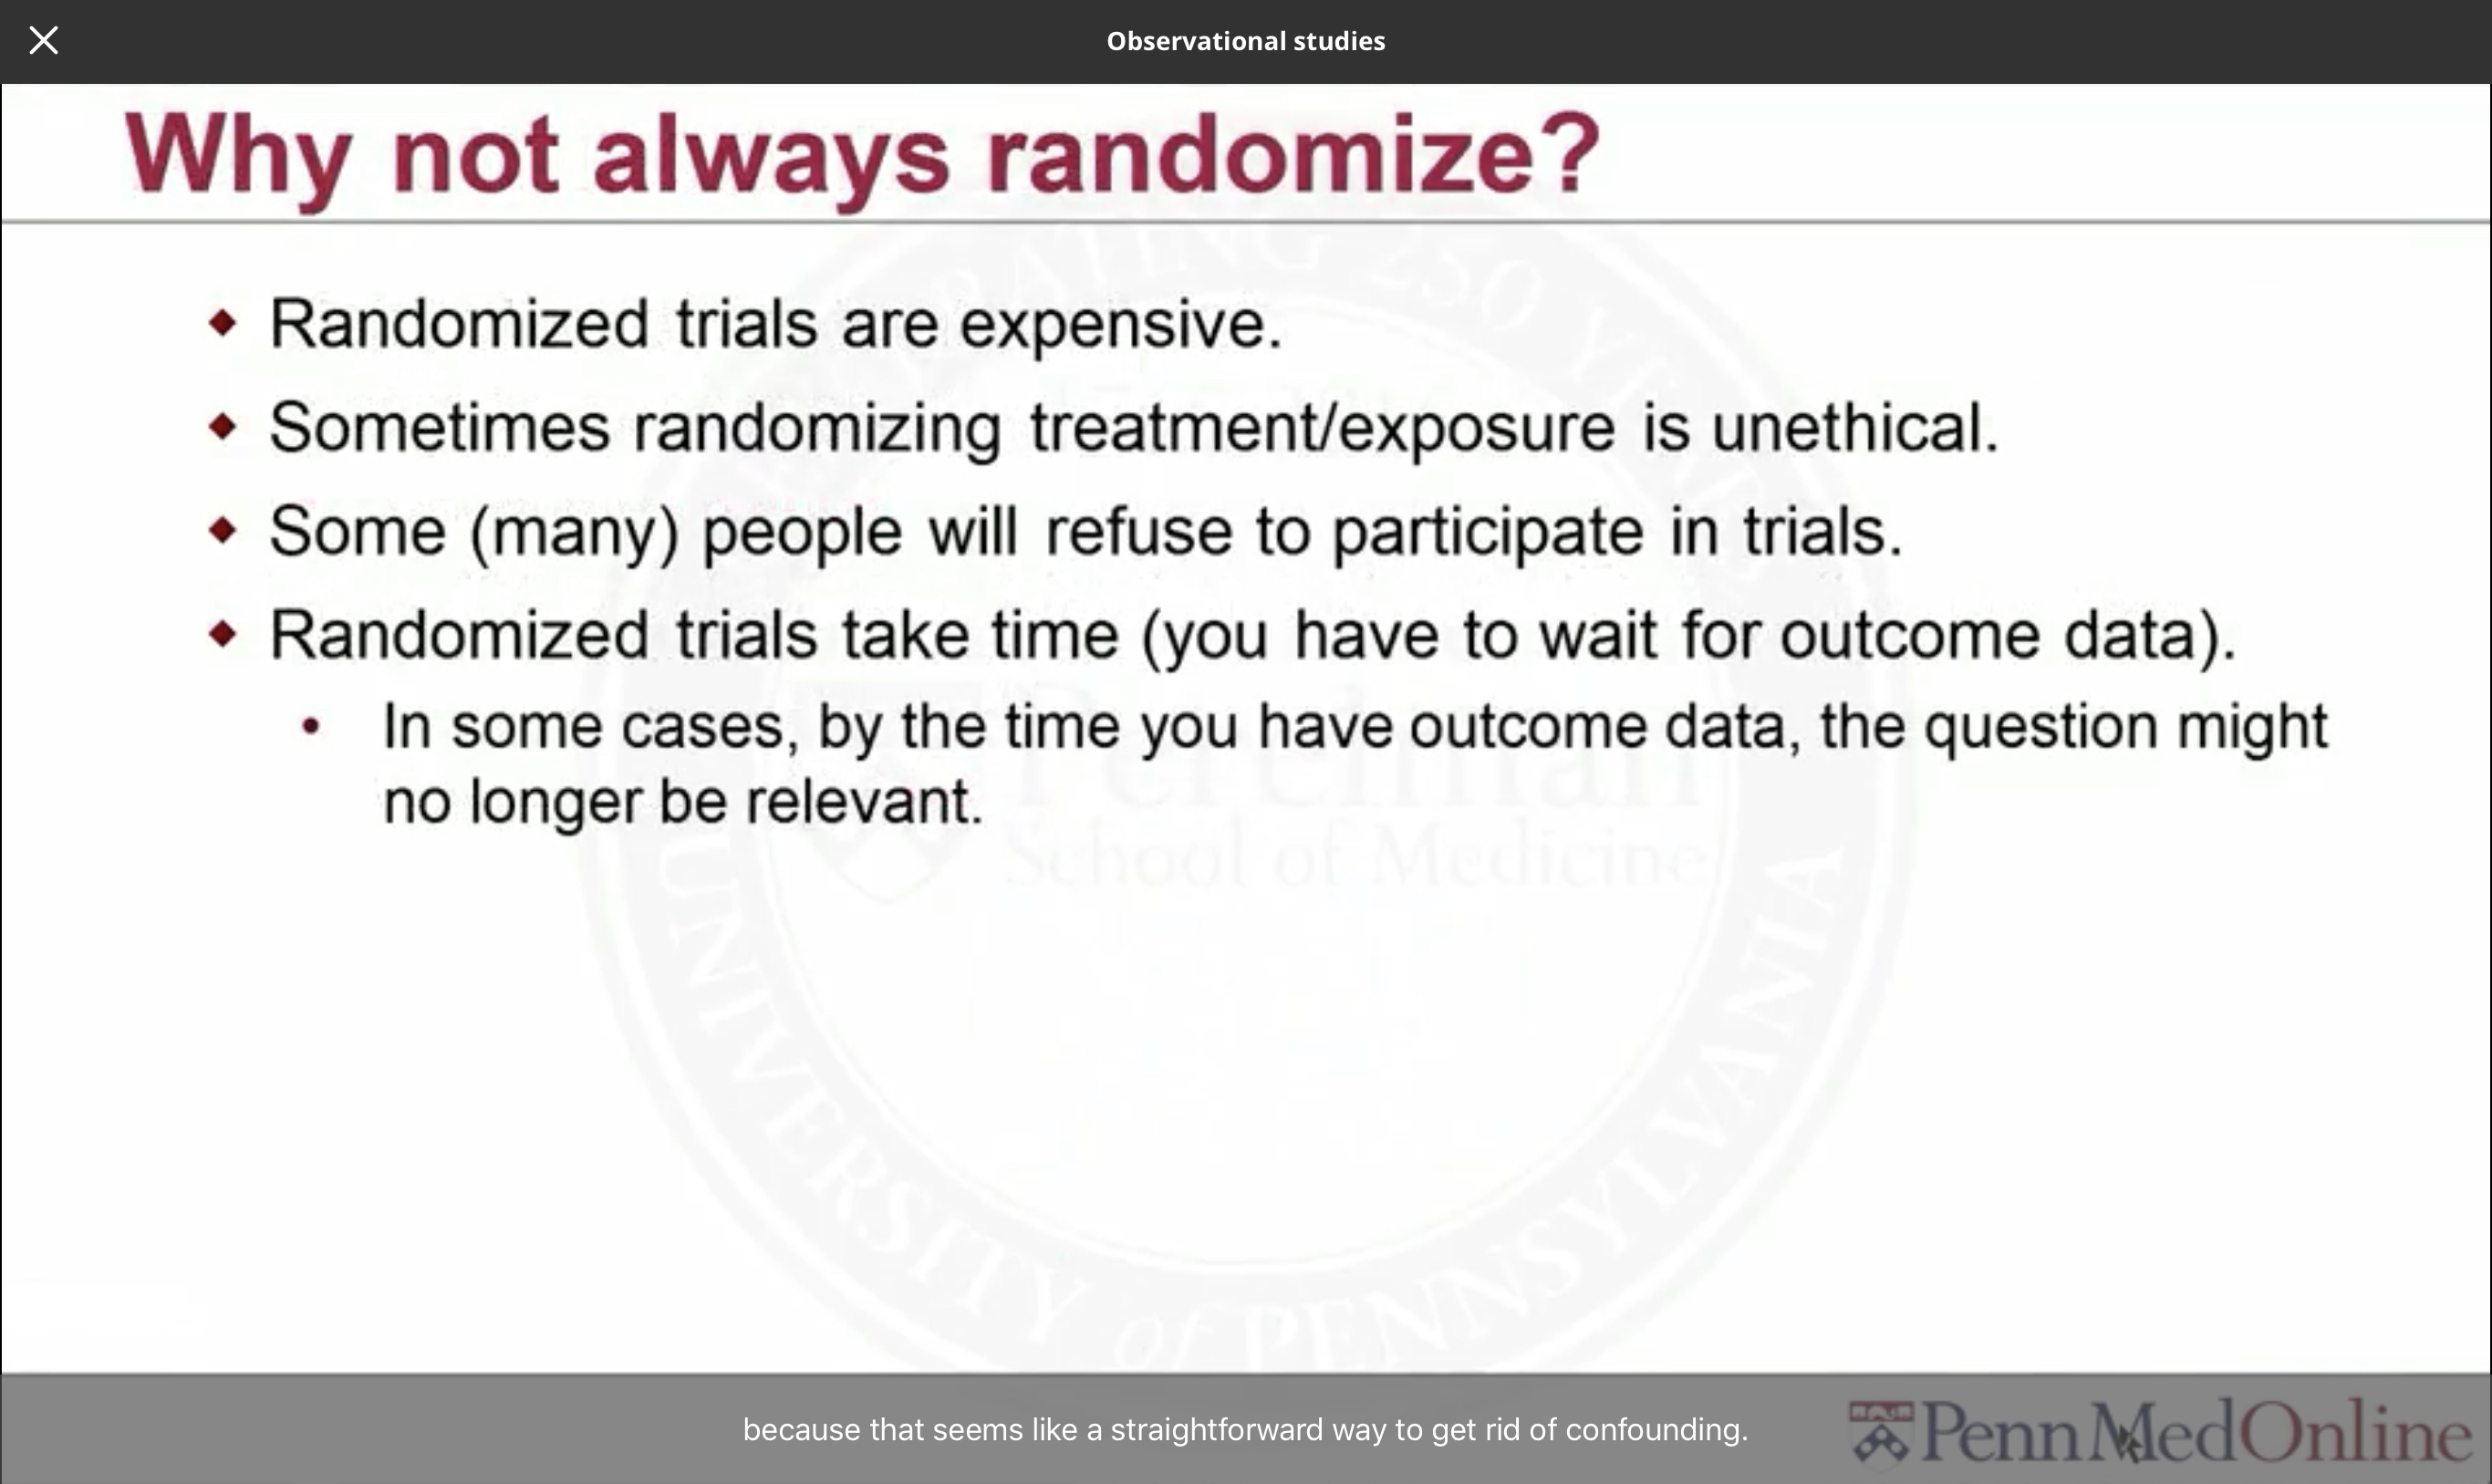
\includegraphics[width=0.8\textwidth]{figure/rmwhynot.jpg}
	\caption{Why not always randomize?}
	\label{rmwhynot}
\end{figure}

\subsection{Recall}
\noindent 1. Classic confounding setting
\begin{itemize}
	\item a set of variable $X$.
	\item $X \rightarrow A$.
	\item $X \rightarrow Y$.
\end{itemize}

在下面两个条件下,控制$X$ is sufficient to control for confounding:
\begin{enumerate}[itemindent=2em,label=(\arabic*)] 
	\item Disjunctive cause criterion.
	\item Backdoor path criterion.
\end{enumerate}

\noindent 2. Ignorability assumption
\begin{equation}
Y^0,Y^1 \perp A|X.
\end{equation}

在给定X后,outcome与处理独立.可以理解为,在X相同的样本中,outcome与是否处理是独立的.


\section{Overview of Matching}
\noindent {\bfseries Outline}:\\
1. Stochastic balance and Fine balance.

\subsection{Single Covariate}
假设只有一个Covariate,可以通过matching达到treated组和control组的perfect match.
\begin{enumerate}[label=(\arabic*)]
	\item Match each treated subject to control subject.
	
	\item Find the best matches and get rid of the subjects who were't matched. 在上一节也说过,我们要去掉那些“have no chance to get another treat"的subjects.
\end{enumerate}

通过Matching,covariate的各取值在treated和control组中的比例都相同,可以达到精准的匹配.

\subsection{Many Covariates}
当有多个covariates的时候,我们不能对所有的covariates都进行perfect match. 即使是在randomized trials的情况下,给定一个treated subject,也可能不存在达成perfect match的single control subject.
此时,randomized trial达到的是一种covariates分布的组间“平衡”,称为{\color{red}{“Stochastic balance”}}.

\begin{ex}
In this example,We have two covaraites:age and gender. There are two subjects in treated group: male aged 56 and female aged 47. \\
\begin{note}
	{\color{orange} \quad Start in treated group, and find people in the control group who are like them.} 
\end{note} 
现在我们在Control group中找一个male subject whose age is similar to 56. 然后再在Control group中找一个female subject whose age is similar to 47. 如Fig.\ref{twocovariates}所示.
\end{ex}

\begin{figure}
	\setlength{\abovecaptionskip}{0pt}     %调整图片标题与图距离
	\setlength{\belowcaptionskip}{10pt}
	\vspace{-0cm}  %调整图片与上文的垂直距离
	\setlength{\abovecaptionskip}{-0cm}   %调整图片标题与图距离
	\setlength{\belowcaptionskip}{-0cm}   %调整图片标题与下文距离
	\centering
	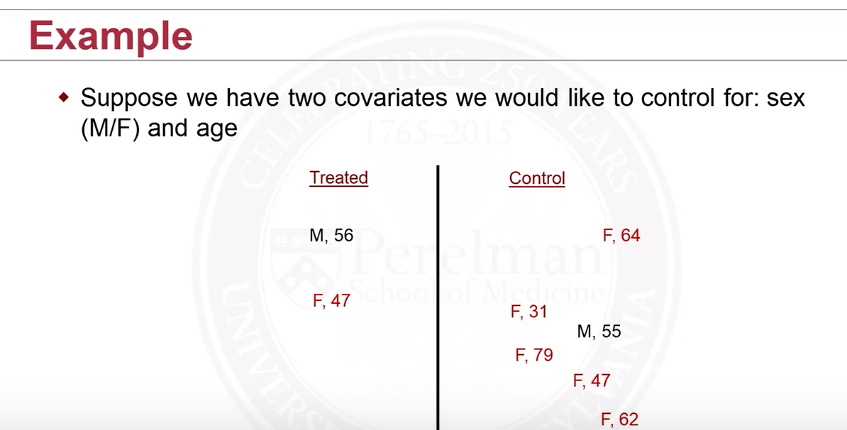
\includegraphics[width=0.8\textwidth]{figure/twocovariates.png}
	\caption{Example:two covariates matching}
	\label{twocovariates}
\end{figure}
在这个过程中,我们是在令control group中的covariates的分布与treated population近似,本质上是求"causal effect of treatment on the treated".

\noindent {\bfseries Remember:}\\
在Matching的过程中,\hl {If we begin with the treated group, and then try to find controls that are good matches for them, you're essentially making inference about the treated population.So you're estimating the "causal effect of treatment on the treated".}

\subsection{Stochastic balance:}
这是一种covariates分布的组间“balance”,“balance”是指confounders在tread group和control group中的分布是相似的. 
\begin{itemize}
   \item Matching {\color{red}{not}} exactly.
   \item Close matches and the distribution of covariates should be {\color{red}{similar}} in two groups.
\end{itemize}


\subsection{Fine balance}
有时候我们不能达到great matching,需要适当放松对matching的要求. 我们可以接受一些non-ideal matching的点,但要求treated和control group中具有the same distribution of covariates. 这种情况称为{\color{red}fine matching}.

\begin{figure}
	\setlength{\abovecaptionskip}{0pt}     %调整图片标题与图距离
	\setlength{\belowcaptionskip}{10pt}
	\vspace{-0cm}  %调整图片与上文的垂直距离
	\setlength{\abovecaptionskip}{-0cm}   %调整图片标题与图距离
	\setlength{\belowcaptionskip}{-0cm}   %调整图片标题与下文距离
	\centering
	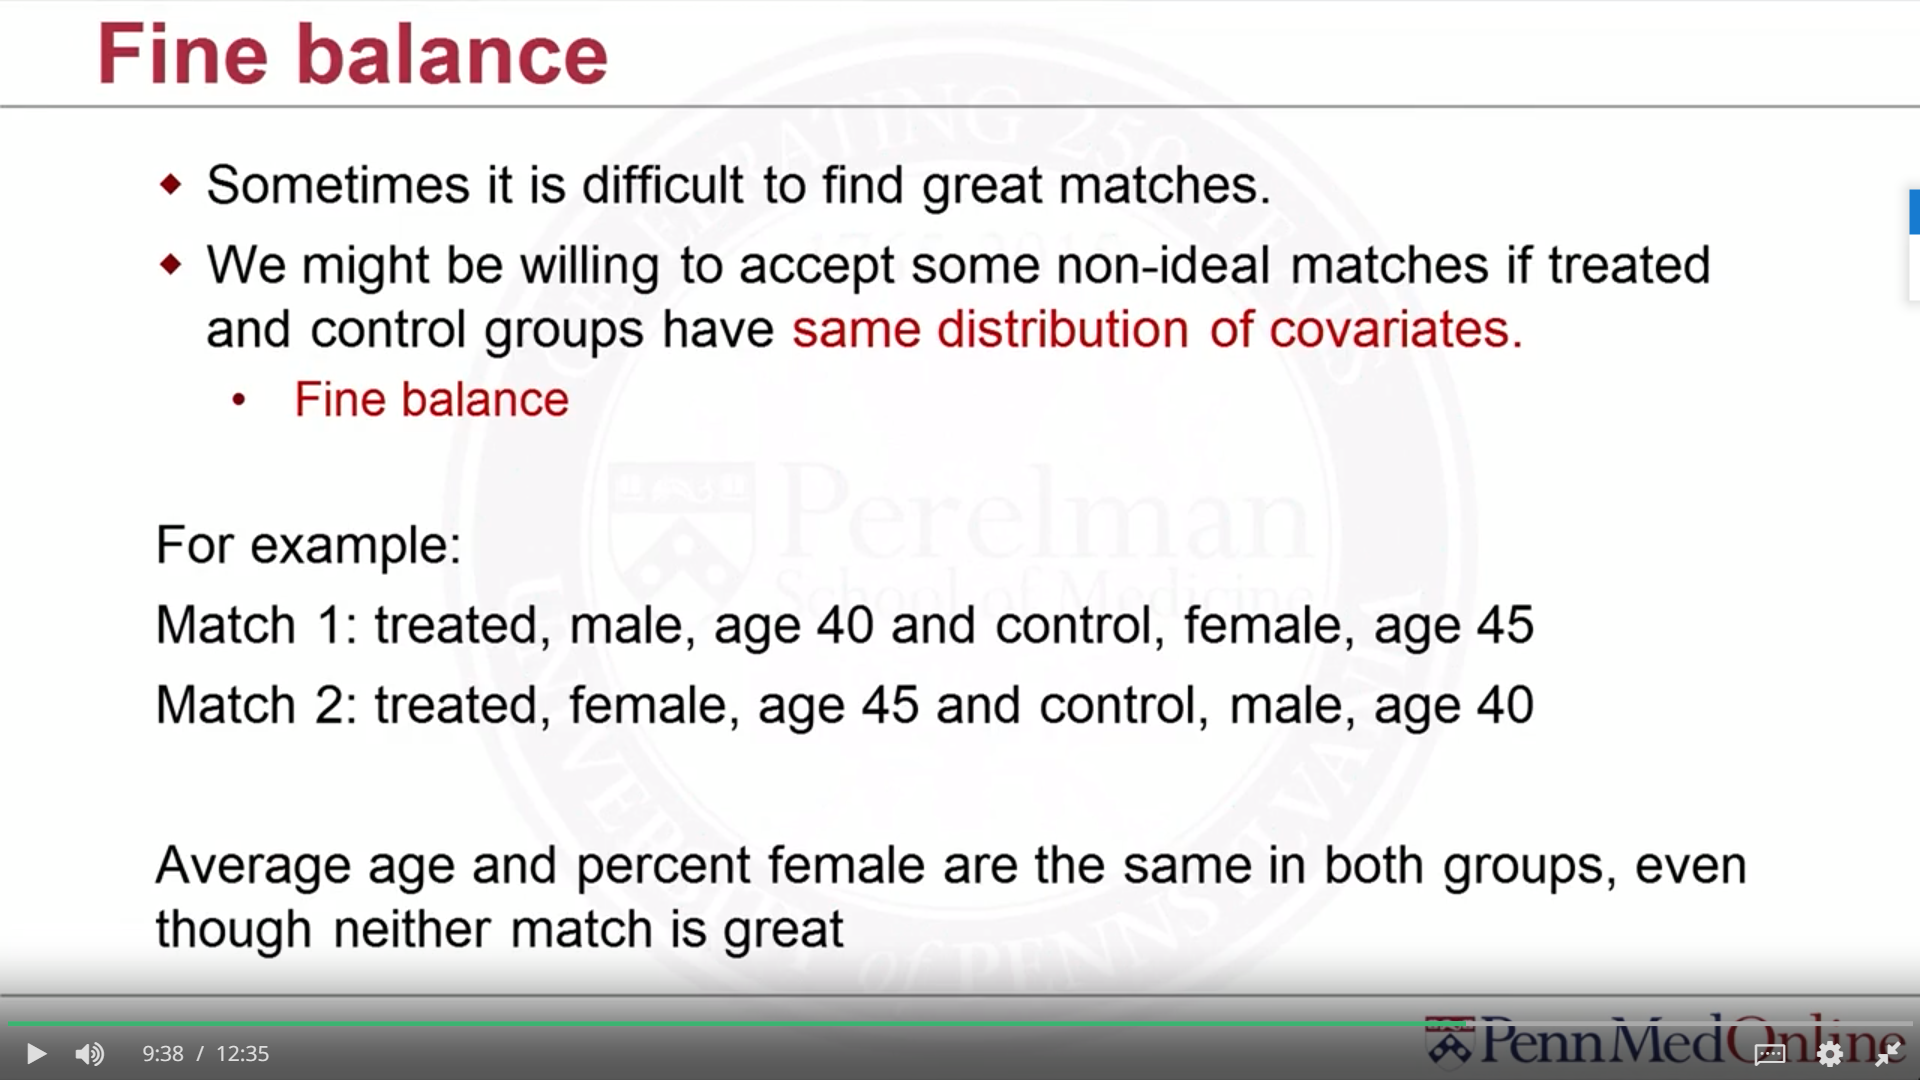
\includegraphics[width=0.8\textwidth]{figure/finebalance.png}
	\caption{Example:Fine balance}
	\label{finebalance}
\end{figure}


\subsection{Number of matches}
\begin{itemize}
	\item[$\blacktriangle$] One-to-one matching: 对于{\color{red}{每一个}}treated subject,都匹配到{\color{red}{一个}}control subject.
	
	\item[$\blacktriangle$] Many to one matching: 对于{\color{red}{每一个}}treated subject,都匹配到{\color{red}{K个}}control subject.
	\item[$\blacktriangle$] Variable matching:对于{\color{red}{每一个}}treated subject,都匹配到{\color{red}{未知个数的}}control subject.
	这依赖于我们可以找到多少对good-matches. 有时候对于一个treated subject可以找到多个good matches,那么就可以全部match上. 
\end{itemize}

当一个treated subject可以找到多个good matches时才可以使用variable matching,如果找不到多个,不要使用.

One-to-one matching的优点就是every pair is good-match. 不过它的缺点也很明显,当一个treated subject可以有多个good-macthes匹配时,只能选择一个good match,其余的controls都丢掉了,这样降低了efficiency.

\newpage \section{Greedy Matching}
\label{greedy}
{\bfseries Outline:}\\
1. What greedy (Nearest-Neighbor) matching is? How the  algorithm works?\\
2. The advantage and disadvantages of greedy matching.\\
3. Many to one matching VS pair matching. Discuss trade-off with the two approaches. \\
4. Introduce the idea of calipers.

\subsection{Set-up}
\begin{itemize}
	\item We have selected a set of pre-treatment covariates X that satisfy the ignorability assupmtion.
	\item We have calculated a distance $d_{ij}$ between each treated subject with every control subject. 计算每一个处理组的对象与每一个控制组的对象之间的距离$d_{ij}$.
\end{itemize}

\subsection{One-to-one Matching}
1. Randomly order list of treated subjects and control subjects.\\
2. {\bfseries Greedy step: find best match.} Start with the 1st treated subjects. Match to the control subject with the smallest distance.\\
3. Remove the matched control from the list of avaliable matches. 匹配过的control subject从候选controls中删掉.\\
4. Move on to the next treated subject. Match to the control with smallest distance.\\
5. Repeat steps 3 and 4 until all treated subjects being matched. \\
{\bfseries R package:MatchIt.}

\subsection{Advantage and Disadvantage}
\begin{itemize}
	\item 容易理解,原理简单.
	\item 计算速度快,计算难度小:逐个计算距离,求最小. 即使对于大型数据计算也很快.
	\item 与treated组的初始排序有关,初始排序不同,得到的匹配也不同.
	\item 不能得到全局最优解:成对的最小距离匹配并不能最小化整个total distance.
	\item 有时会因为别无选择导致bad matches,瘸子里挑将军.
\end{itemize}

\subsection{Many-to-one Matching}
For K:1 matching: after everyone has 1 match, go through the list again and find 2\ts{nd} matches. Repeat until k matches.

\subsection{Trade-off between 1-1 and k-1}
\begin{enumerate}[itemindent=2em,label=(\arabic*)] 
	\item Pair matching进行的匹配误差(bias)更小,但是多余的control subjects都被丢掉了,所以损失了一部分效率,引入了更大的variance. 当然可以通过增加treated subjects增加匹配,减少control subjects损失,不过能弥补回来的效率并不多. 它的优点是计算速度很快.
	\item Many-to-one match进行的匹配误差(bias)更大,但是variance更小. 
\end{enumerate}
所以在这两者之间可以进行一个trade-off.

\subsection{caliper}
在Greedy matching算法中,有些匹配是很差的,所以如果想要更好的匹配,就可以设置一个距离的上限,使得超过这个上限的匹配都被舍弃. 这个可接受的最大距离就称为Caliper.
\begin{itemize}
	\item Go through the greedy matching.
	\item Get rid of the matches which disance greater than caliper.
\end{itemize}

Positivity assumption: Probability of each treatment given X should be non-zero.
对于一个treated subject,如果在caliper的限制下找不到good match的话,说明这个treated subject没有可能被分到control组,这样就违背了positivity assumption. 一个解决方法就是,删除这些subjects. 

\section{Optimal Matching}
\label{optimal}
\subsection{Greedy matching is not optimal}
Global optimal: Minimize the total distance of all matched pairs.
\subsection{Computationally Demanding}
1.Do every possible combination and caculate the total distance. \\
2. Choose the matches that have the smallest total distance.

这种方法的困难在于,计算量非常大,对于所有subjects的每一种匹配方式都要算出total distance. 一种计算方法是{\bfseries Network flow optimization approach}. 相关的R包有optmatch和rcbalance. 

Optimal matching是否可解在于subjects的多少,在于the size of the problem. Size表示可能的treated-control pairs的数量, 比如有10000个treated patients和100000个control patients,那么可能的pairs数量为$10^{9}$,因此求解是不可行的.
 
\subsection{Sparse optimal matching(2015, JASA)}
可以提出一些条件,减少可能的匹配数量. 比如有10家医院,在每一家医院内部对病人进行Optimal matching,这样就缩小了匹配的pairs数量. 或者按照其他准则划分blocks,在每个block内部optimize.
Mismatches can be tolerated if fine blance can still achieved.

\section{Assessing Matching}
\label{assessmatch}
{\bfseries Outline:}\\
1. 假设检验:检验treated group与control group的均值是否相同.\\
2. 计算matching前后,每个covariate的Standardized difference. 

\subsection{检验Matching是否成功}
\begin{enumerate}[itemindent=2em,label=(\arabic*)] 
	\item {\bfseries 标准:}treated group 与control group的covariates是否达到一致(Covariate balance)?
	\item {\bfseries 目标:}Covariate在treated与control group中的均值是否相等?
\end{enumerate}

\subsection{检验方法}
1. 假设检验: 两样本t检验,考察p值.
\begin{itemize}
	\item 缺点:p值依赖于样本大小. 在样本大的时候,可能很小的均值差异就会导致p值很小,从而拒绝原假设,认为两组均值不相等.
\end{itemize}

2. 计算标准差异(Standardized difference):
\begin{equation}
smd= \frac{\overline{X}_{t}-\overline{X}_{c}}{\sqrt{\frac{S_{t}^{2}+S_{c}^{2}}{2}}}
\end{equation}
当smd$<$0.01时,我们认为当前covariate的均值在两个组中是没有差异的. 如果smd$>$0.02,就可以认为当前covariate的均值是有差异的,也就违背了causal effect的关键,需要重新Matching.
\begin{note}
Causal Effect的关键:
针对同样的population分别进行treated和control,而不能针对不同的subpopulation进行treated和control,在现实中为了逼近这样的效果,我们通常会令两组subpopulation足够相似,在每个covariate上的分布都相似.
\end{note}

\section{Analyzing data after matching}
前几课已经讨论了如何做Matching(Section \ref{greedy}和Section \ref{optimal})、如何检验matching是否正确(Section \ref{assessmatch}). 那么当检验出Matching成功后,我们需要做的就是对比Matching后treated group和control group的outcome是否有明显差异. 也就是检验是否存在Causal effect(Treatment effect).

\subsection{Permutation test}
Permutation test也称作Randaomized test Or Exact test.
下面我们通过Fig.\ref{pertest}说明Permutation test的基本思想和流程:
\begin{figure}
	\setlength{\abovecaptionskip}{0pt}     %调整图片标题与图距离
	\setlength{\belowcaptionskip}{10pt}
	\vspace{-0cm}  %调整图片与上文的垂直距离
	\setlength{\abovecaptionskip}{-0cm}   %调整图片标题与图距离
	\setlength{\belowcaptionskip}{-0cm}   %调整图片标题与下文距离
	\centering
	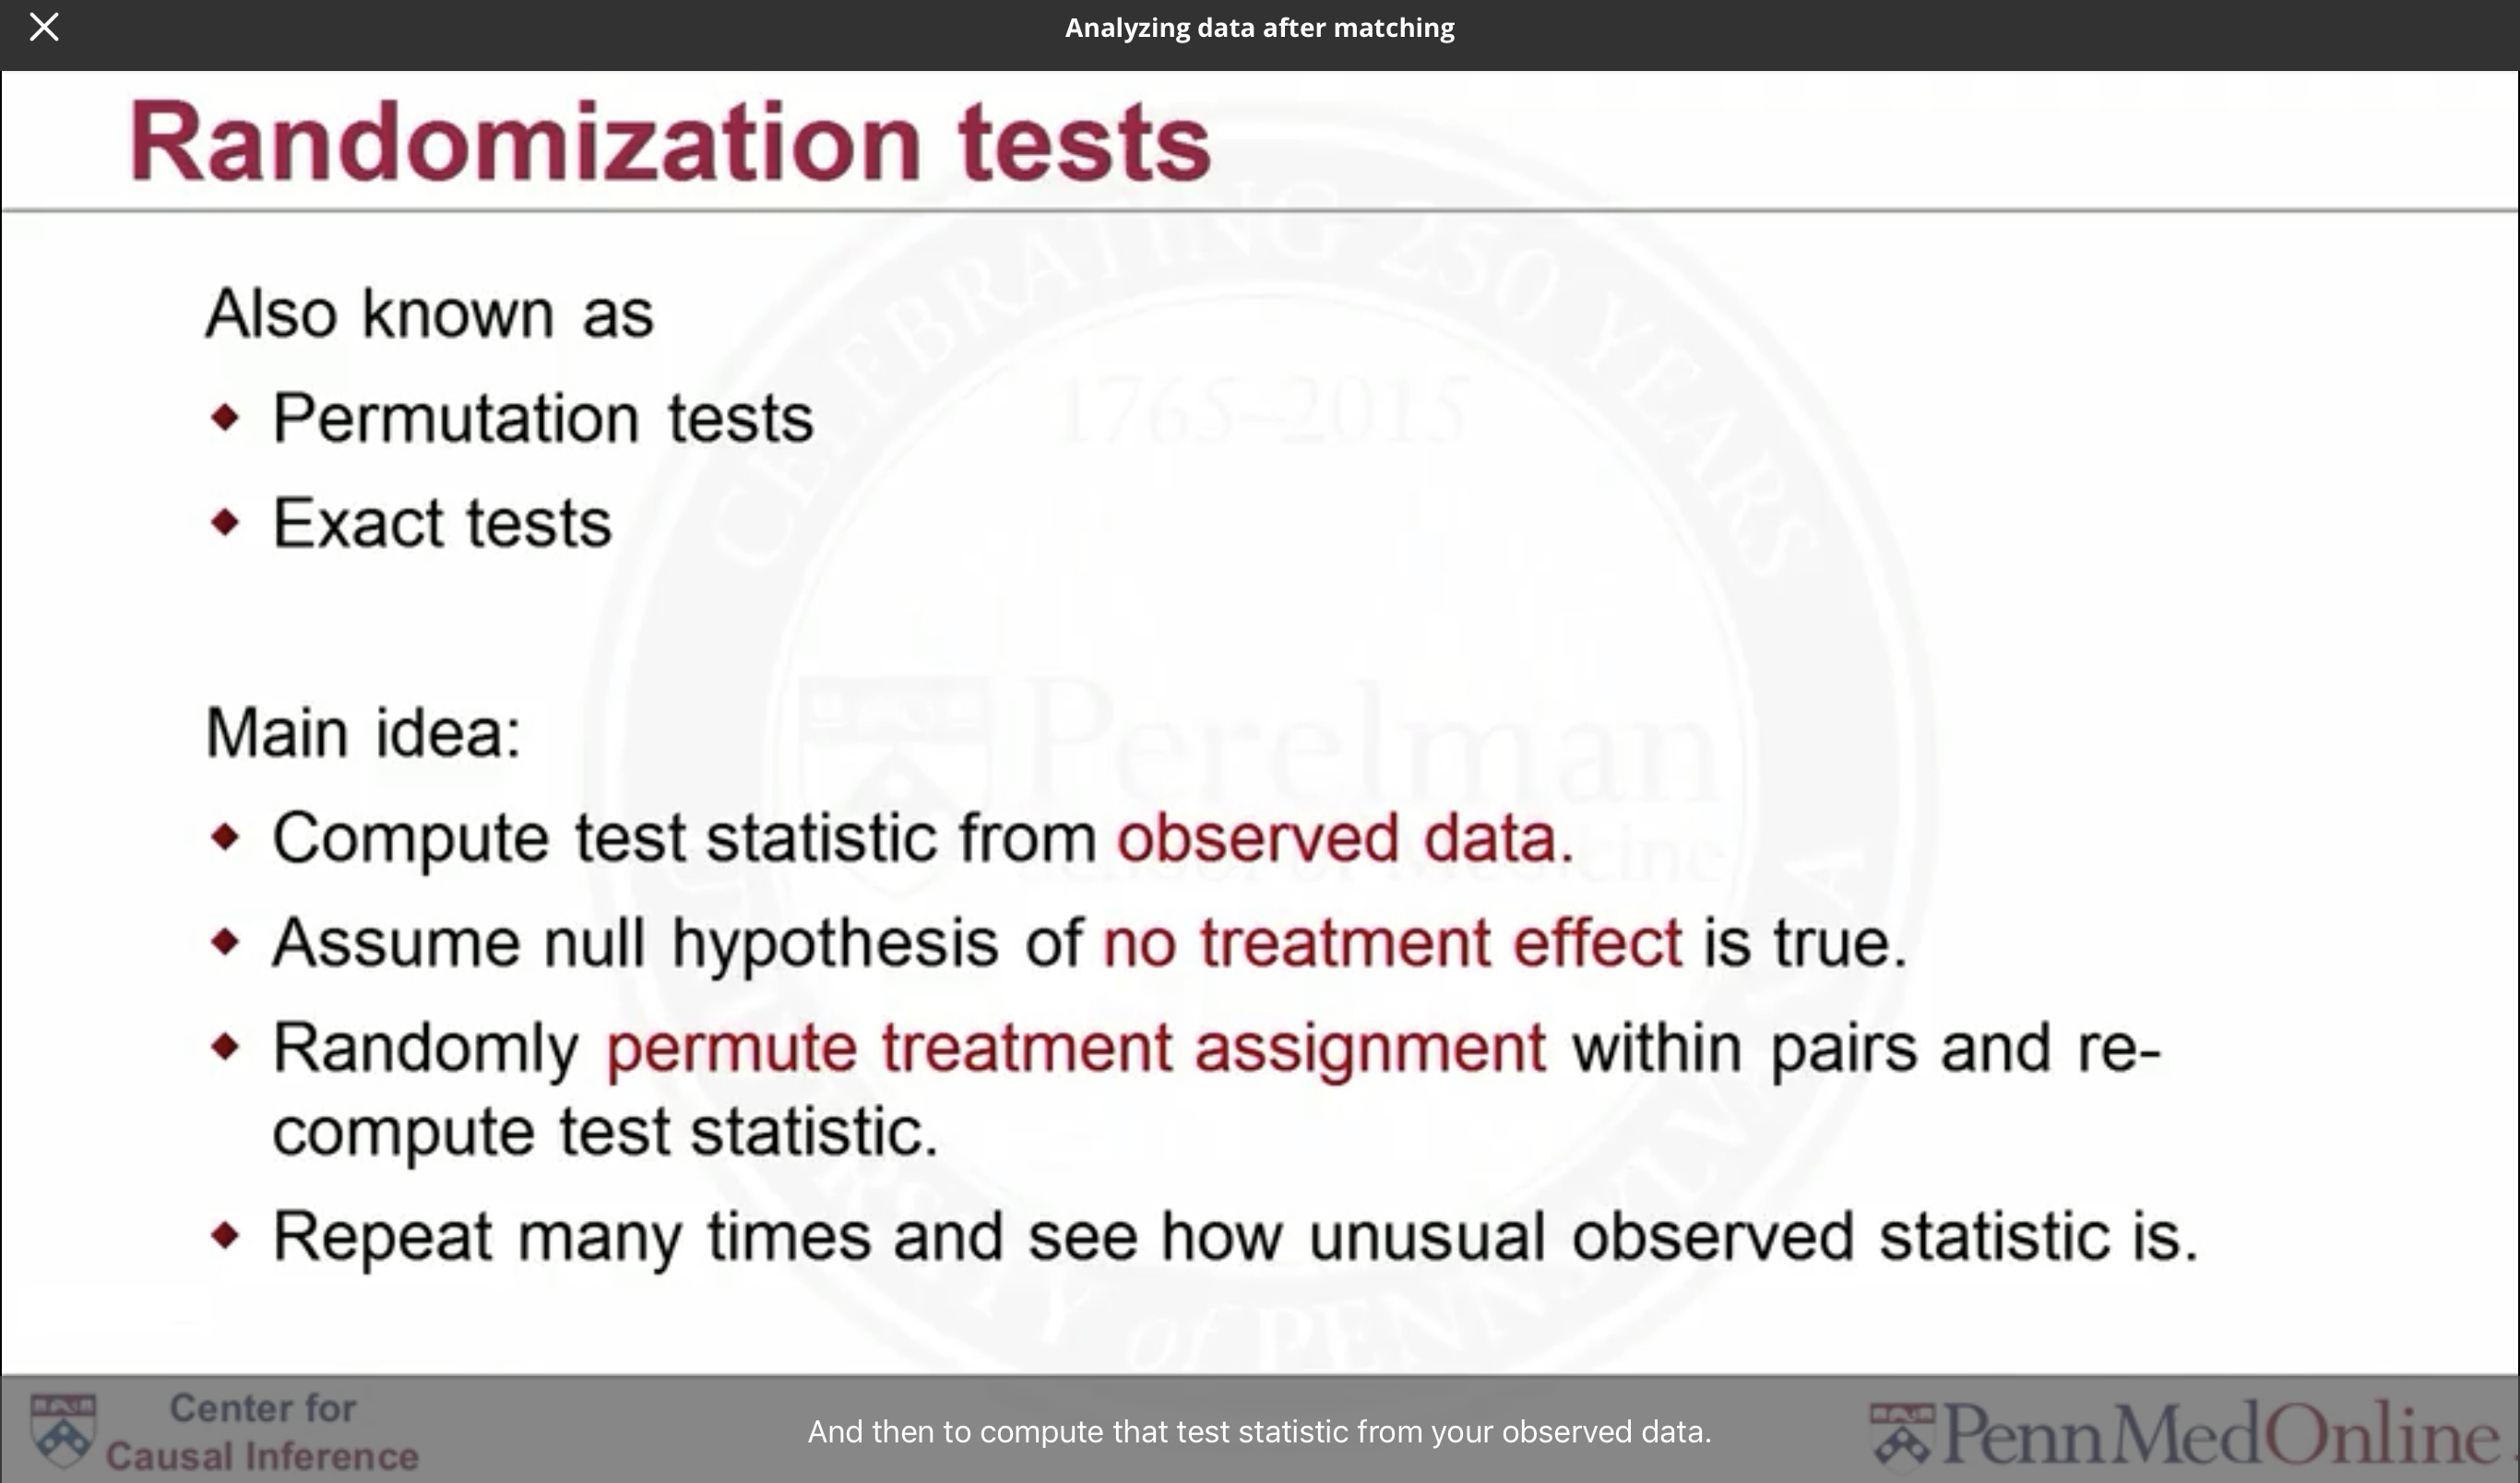
\includegraphics[width=0.8\textwidth]{figure/pertest.jpg}
	\caption{Permutation test}
	\label{pertest}
\end{figure}

Permutation test的思想很简单:构建一个检验统计量,做假设检验. {\bfseries 假设原假设成立},对比original data的test statistic与交换treatment后的permutation data的test statistic是否有明显的差异.
\subsection{Calculation of test statistics}
对于binary outcome,我们可以简单把test statistic取为treated组outcome=1的计数,如Fig.\ref{exper}.
\begin{figure}
	\setlength{\abovecaptionskip}{0pt}     %调整图片标题与图距离
	\setlength{\belowcaptionskip}{10pt}
	\vspace{-0cm}  %调整图片与上文的垂直距离
	\setlength{\abovecaptionskip}{-0cm}   %调整图片标题与图距离
	\setlength{\belowcaptionskip}{-0cm}   %调整图片标题与下文距离
	\centering
	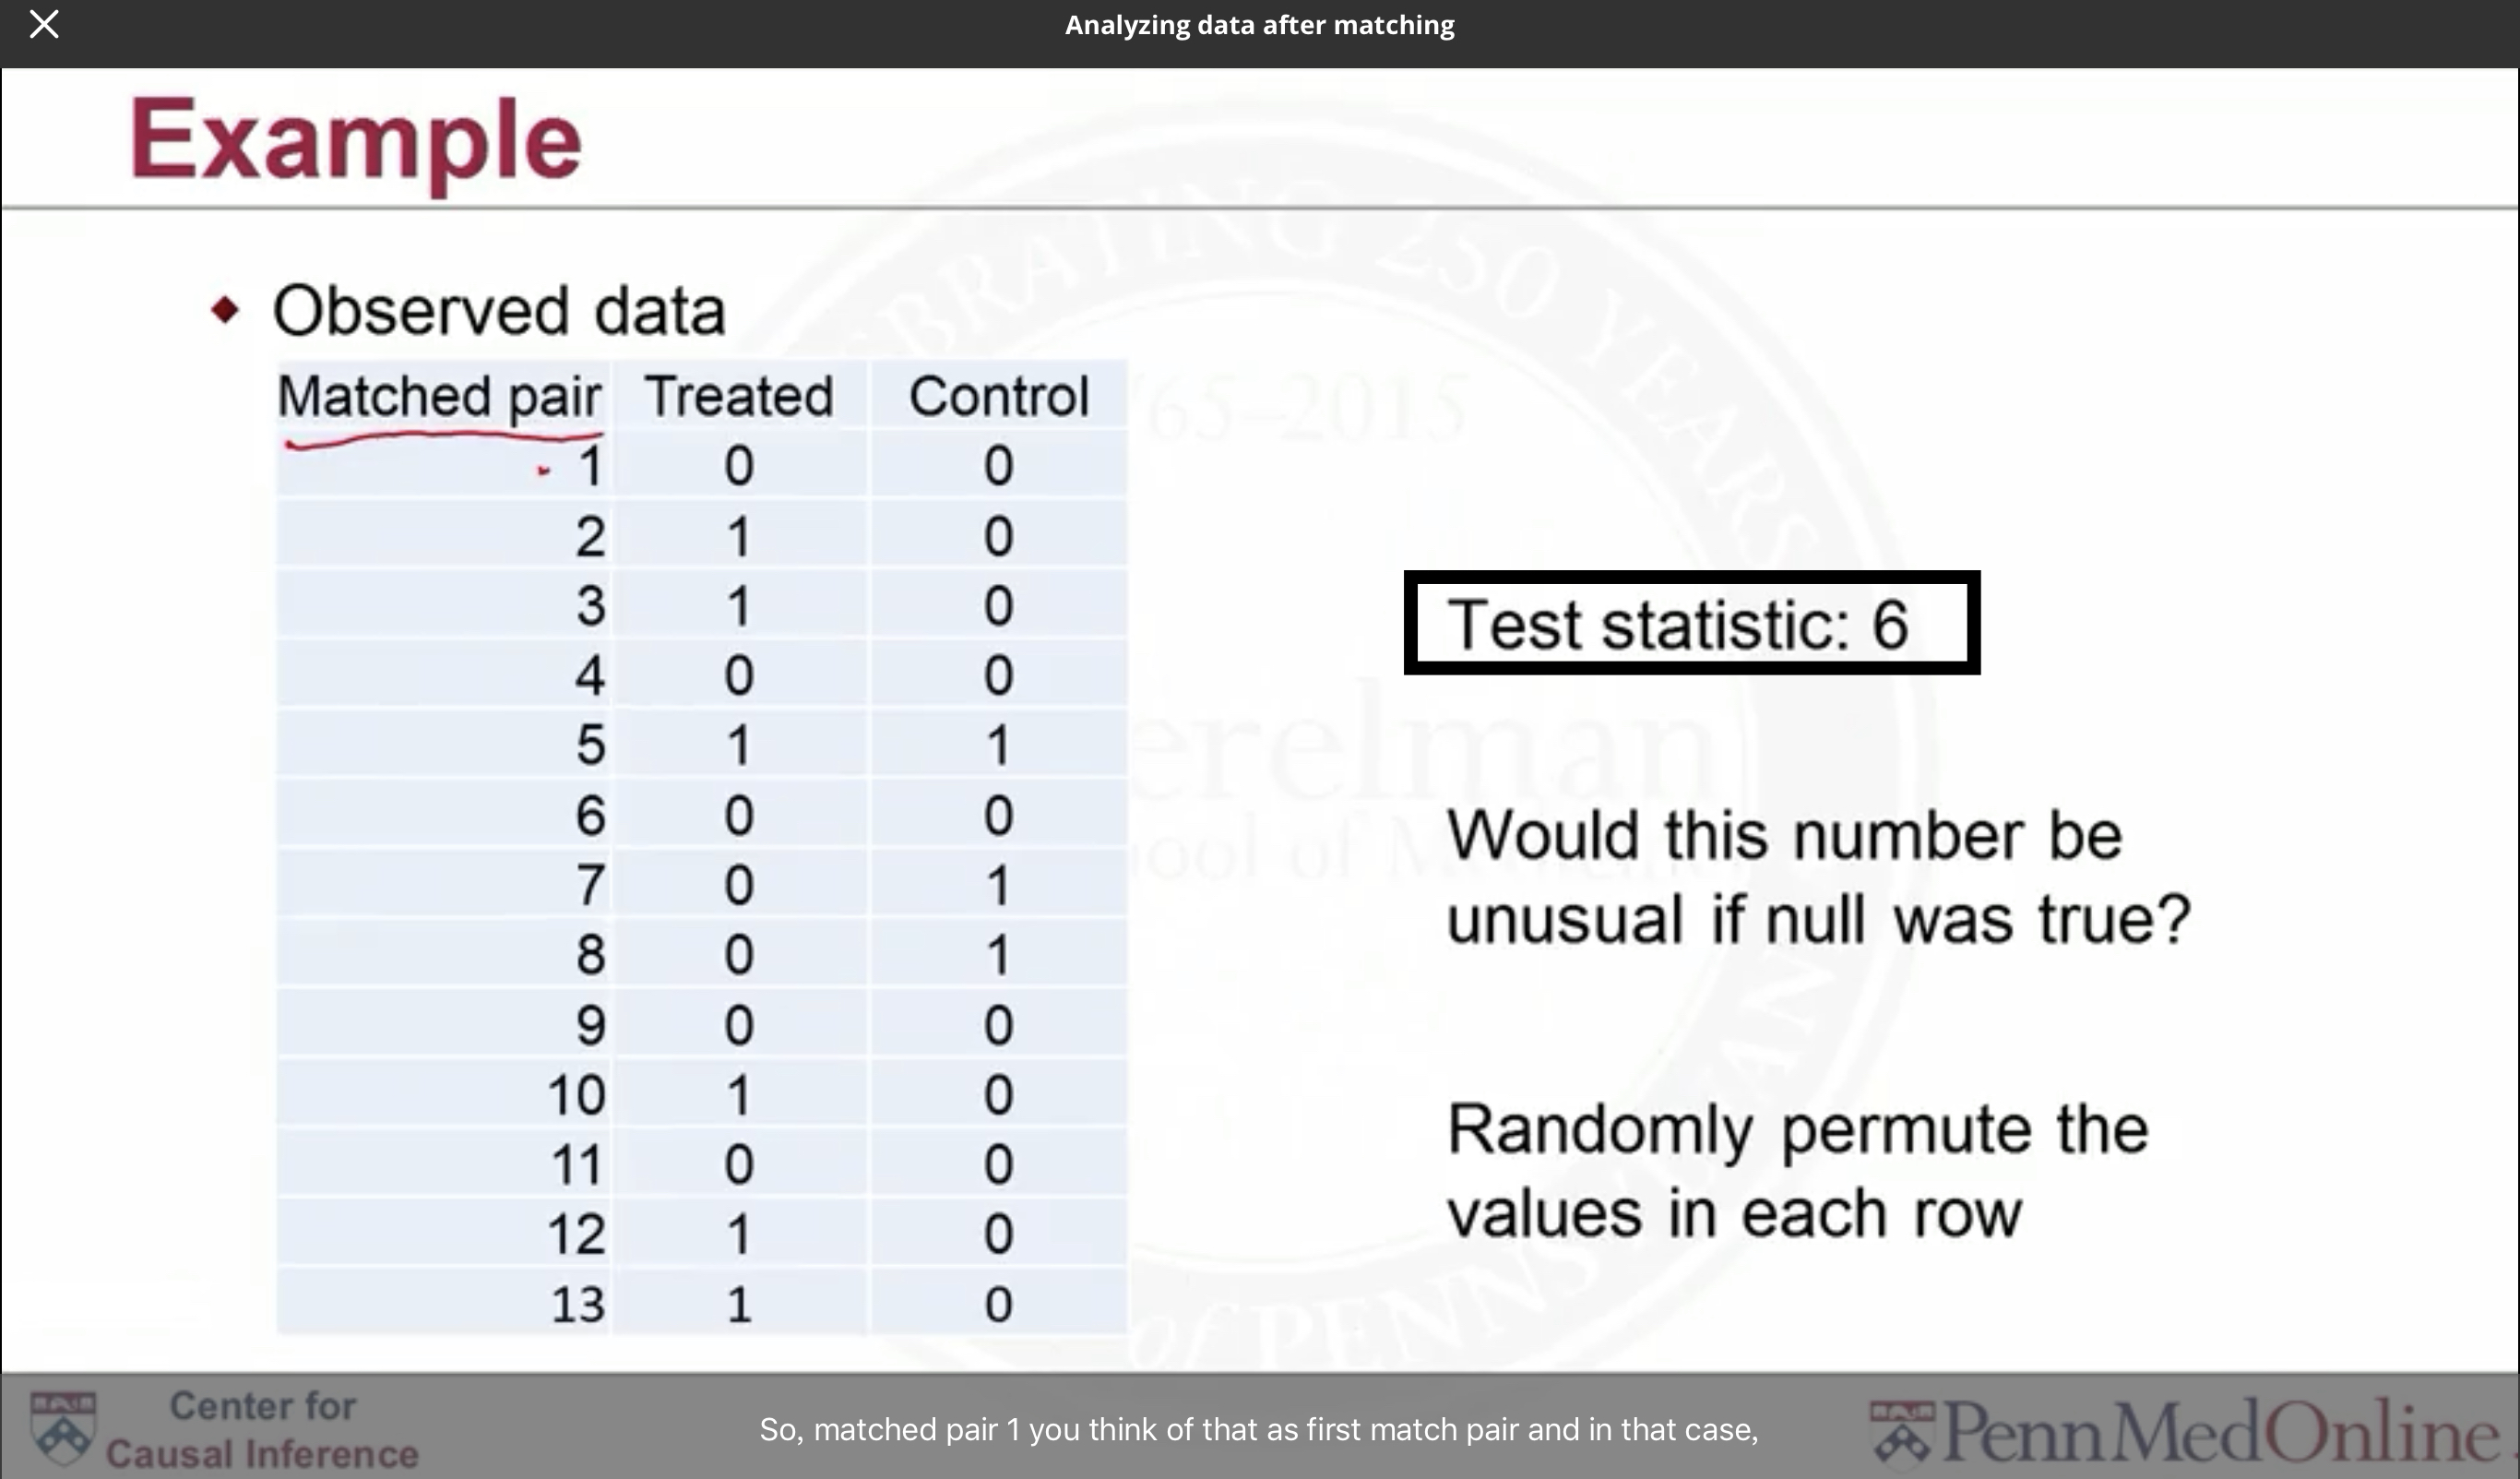
\includegraphics[width=0.8\textwidth]{figure/exper.jpg}
	\caption{Calculation of test statistics}
	\label{exper}
\end{figure}

当然,只进行一次或几次Permutation change可能有偶然性,所以交换treatment的操作可以循环重复K次,然后绘制出test statistics的分布直方图,看统计量集中在哪里. 找出observed data的test statistic,看其是否出现在直方图的集中位置. 

\subsection{Calculation of p value}
或者可以通过计算p值来决定是否接受原假设. p值代表的是在原假设成立的情况下大于观察值或比观察值更极端情况出现的概率. 以Fig.\ref{histts}为例,p值就是将observed data value大于等于6(6,7,8),以及极端值1,2,3出现的概率相加:
\begin{figure}[htbp]
	\setlength{\abovecaptionskip}{0pt}     %调整图片标题与图距离
	\setlength{\belowcaptionskip}{10pt}
	\vspace{-0cm}  %调整图片与上文的垂直距离
	\setlength{\abovecaptionskip}{-0cm}   %调整图片标题与图距离
	\setlength{\belowcaptionskip}{-0cm}   %调整图片标题与下文距离
	\centering
	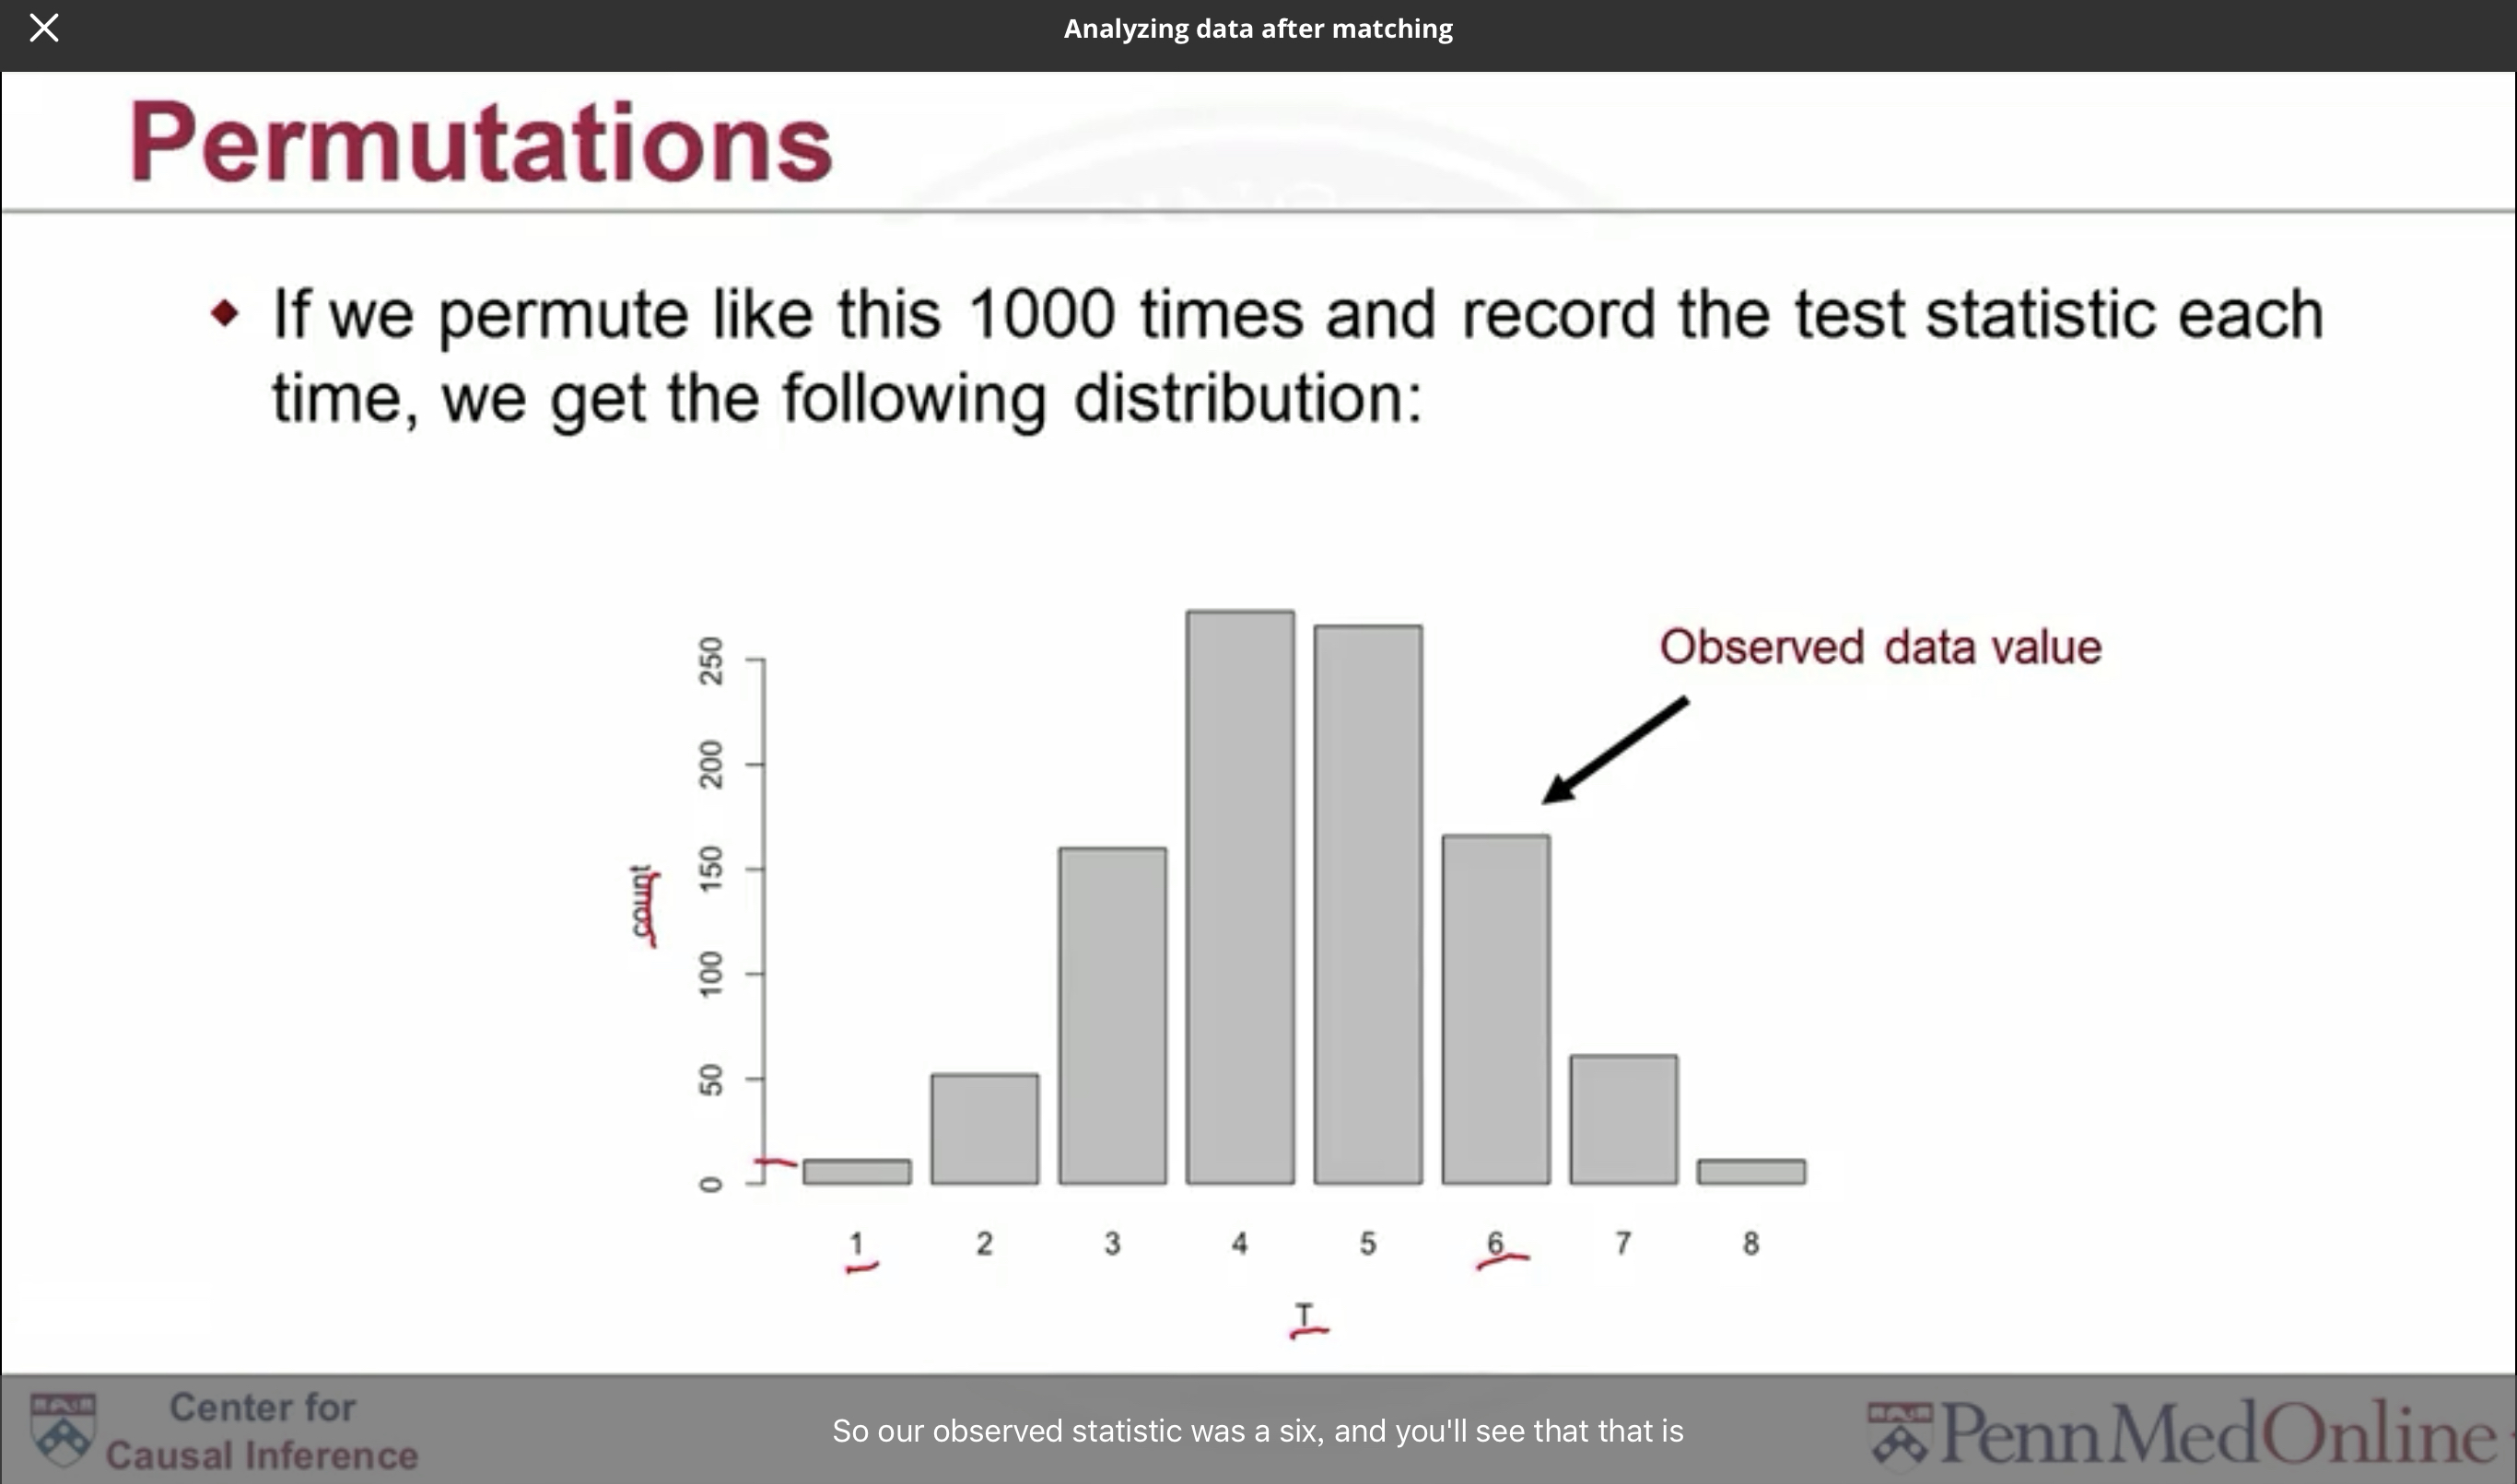
\includegraphics[width=0.8\textwidth]{figure/histts.jpg}
	\caption{Histogram test statistics}
	\label{histts}
\end{figure}

\subsection{Discordant pair}
对于binary outcome来说,交换treated与control只对不一致的pair起作用,对于相同outcome的pair,交换也不会带来什么改变. 

\subsection{McNemar test}
画一个格子点表格,分别计数"Count(outcome=1$|$A=1)","Count(outcome=1$|$A=0)","Count(outcome=0$|$A=1)","Count(outcome=0$|$A=0)". 然后在R中进行mcmemar.test.

\begin{figure}[htbp]
	\setlength{\abovecaptionskip}{0pt}     %调整图片标题与图距离
	\setlength{\belowcaptionskip}{10pt}
	\vspace{-0cm}  %调整图片与上文的垂直距离
	\setlength{\abovecaptionskip}{-0cm}   %调整图片标题与图距离
	\setlength{\belowcaptionskip}{-0cm}   %调整图片标题与下文距离
	\centering
	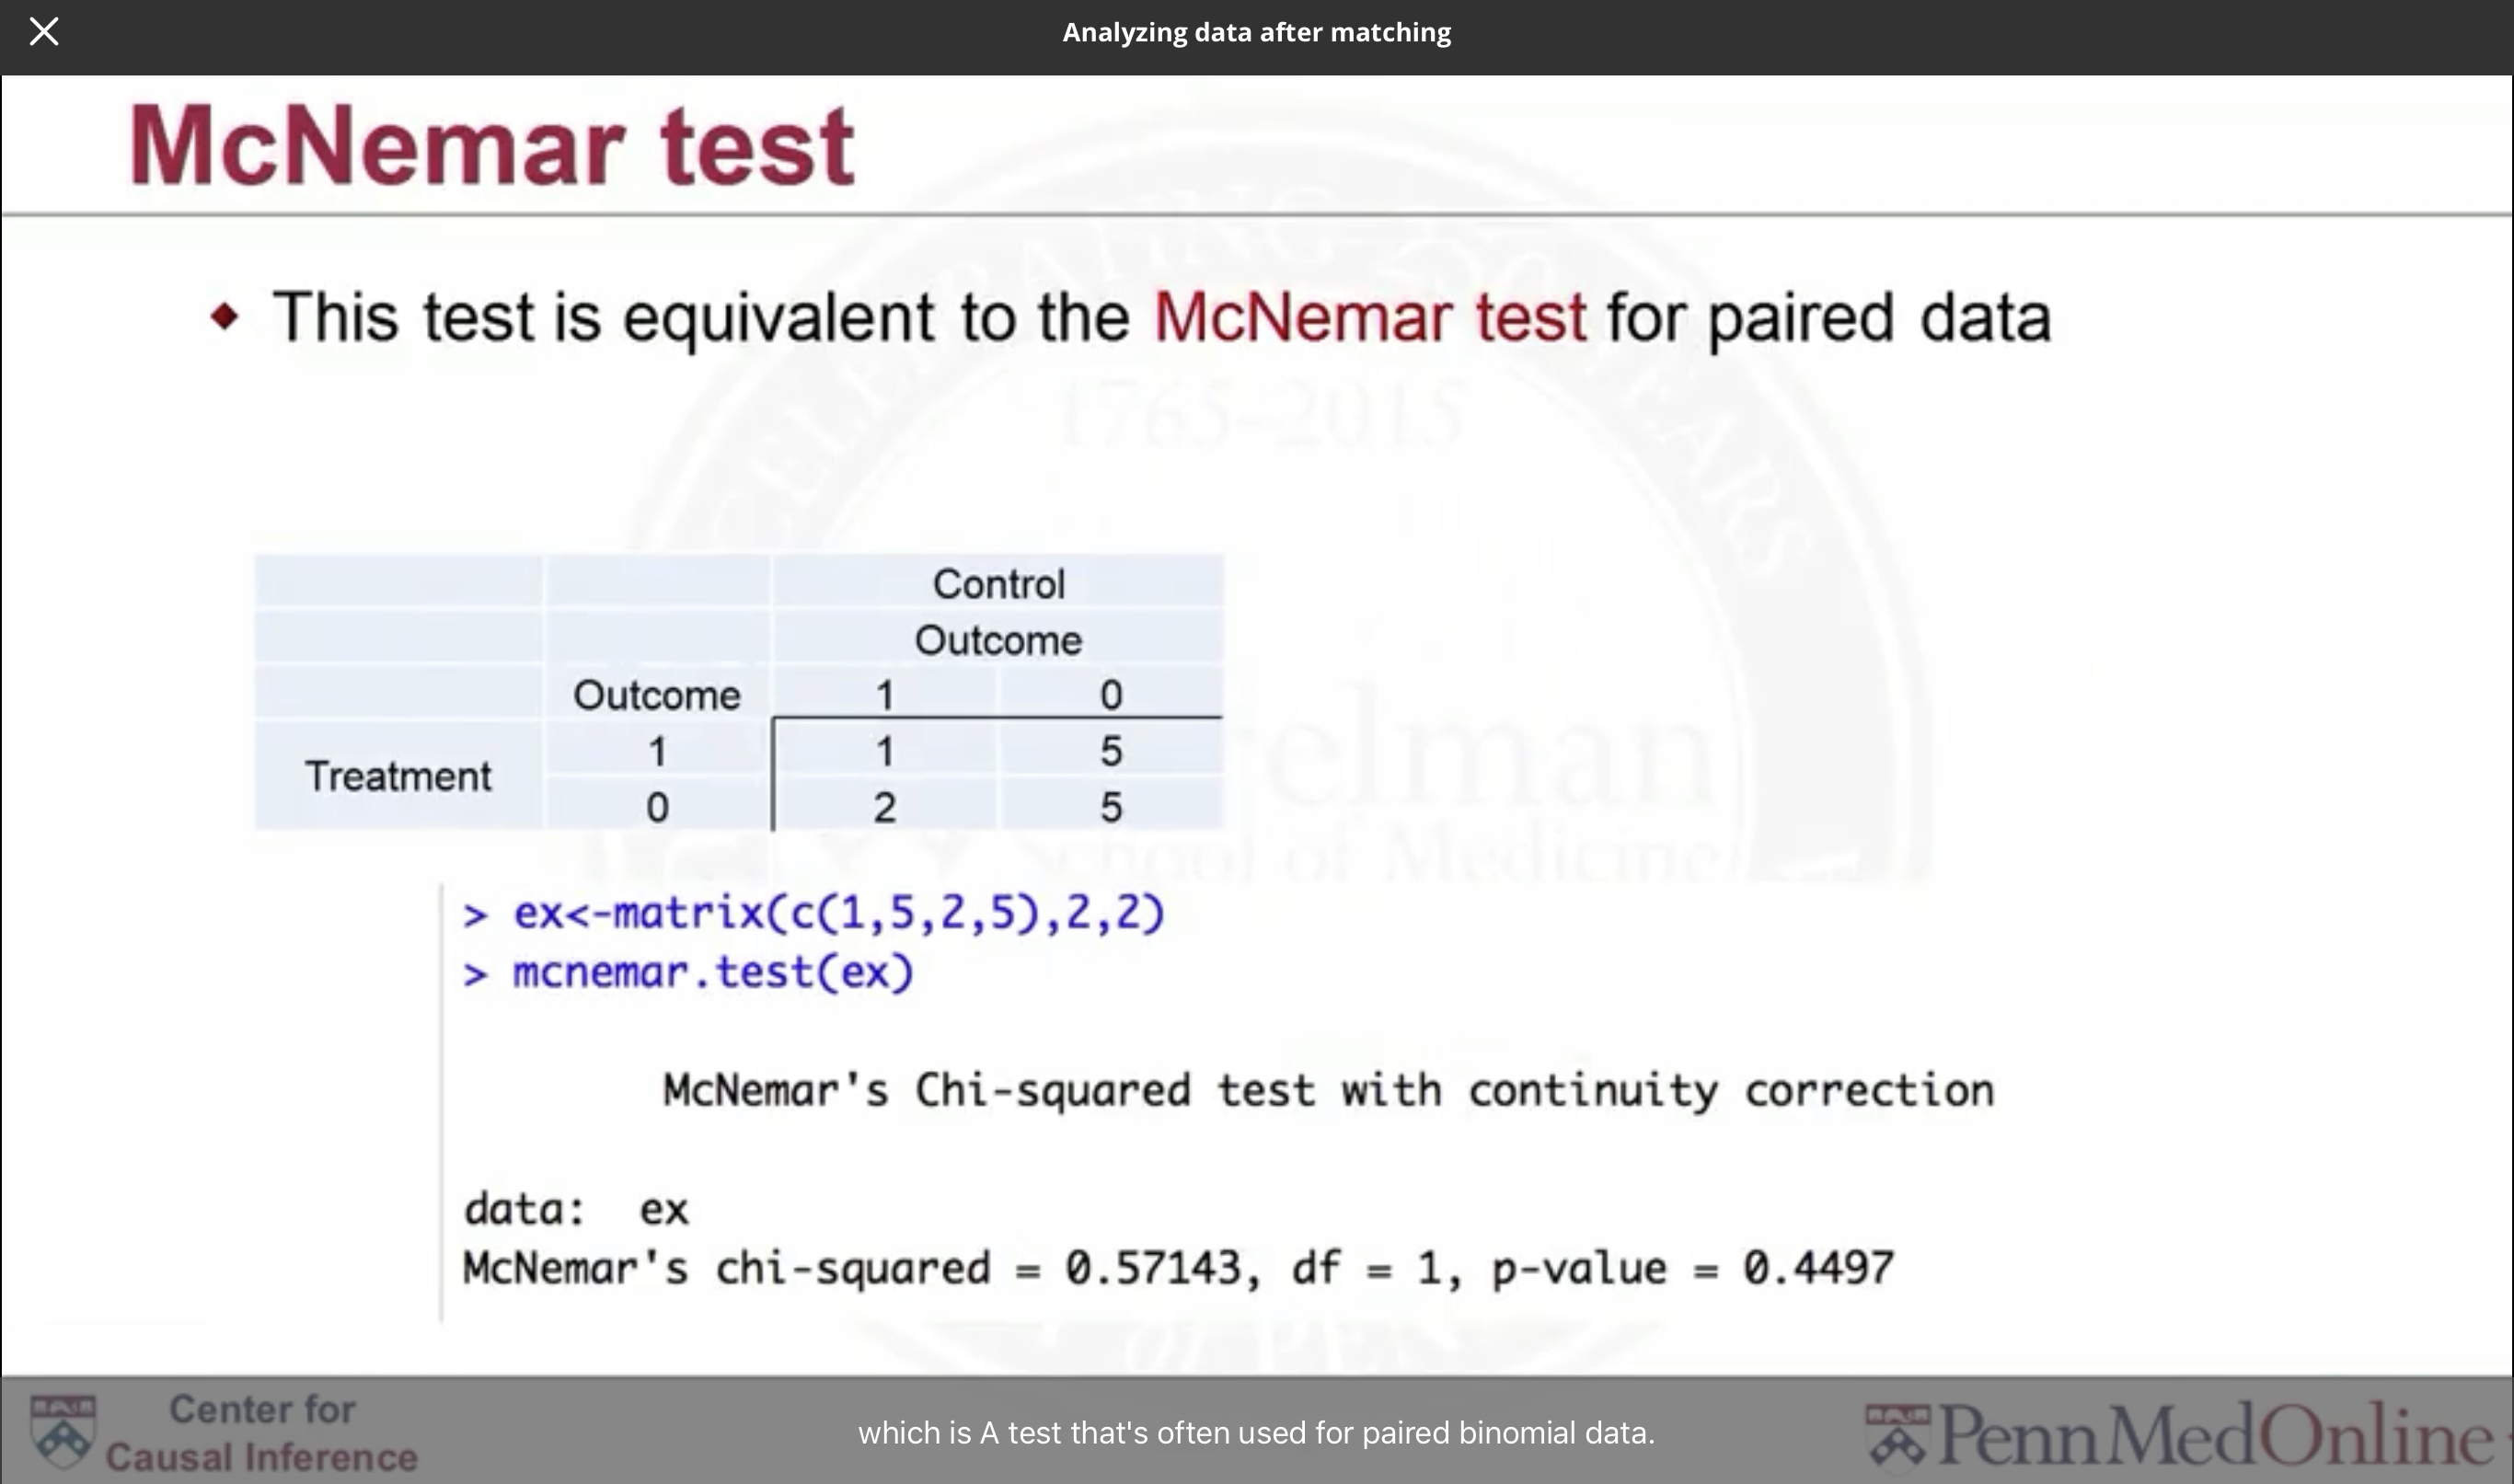
\includegraphics[width=0.8 \textwidth]{figure/mcnemar.jpg}
	\caption{McNemar test}
	\label{mcnemar}
\end{figure}

\section{Sensitivity analysis}
\section{Propensity score}
\section{Propensity score matching}
\section{Data Example: Propensity score match i R}

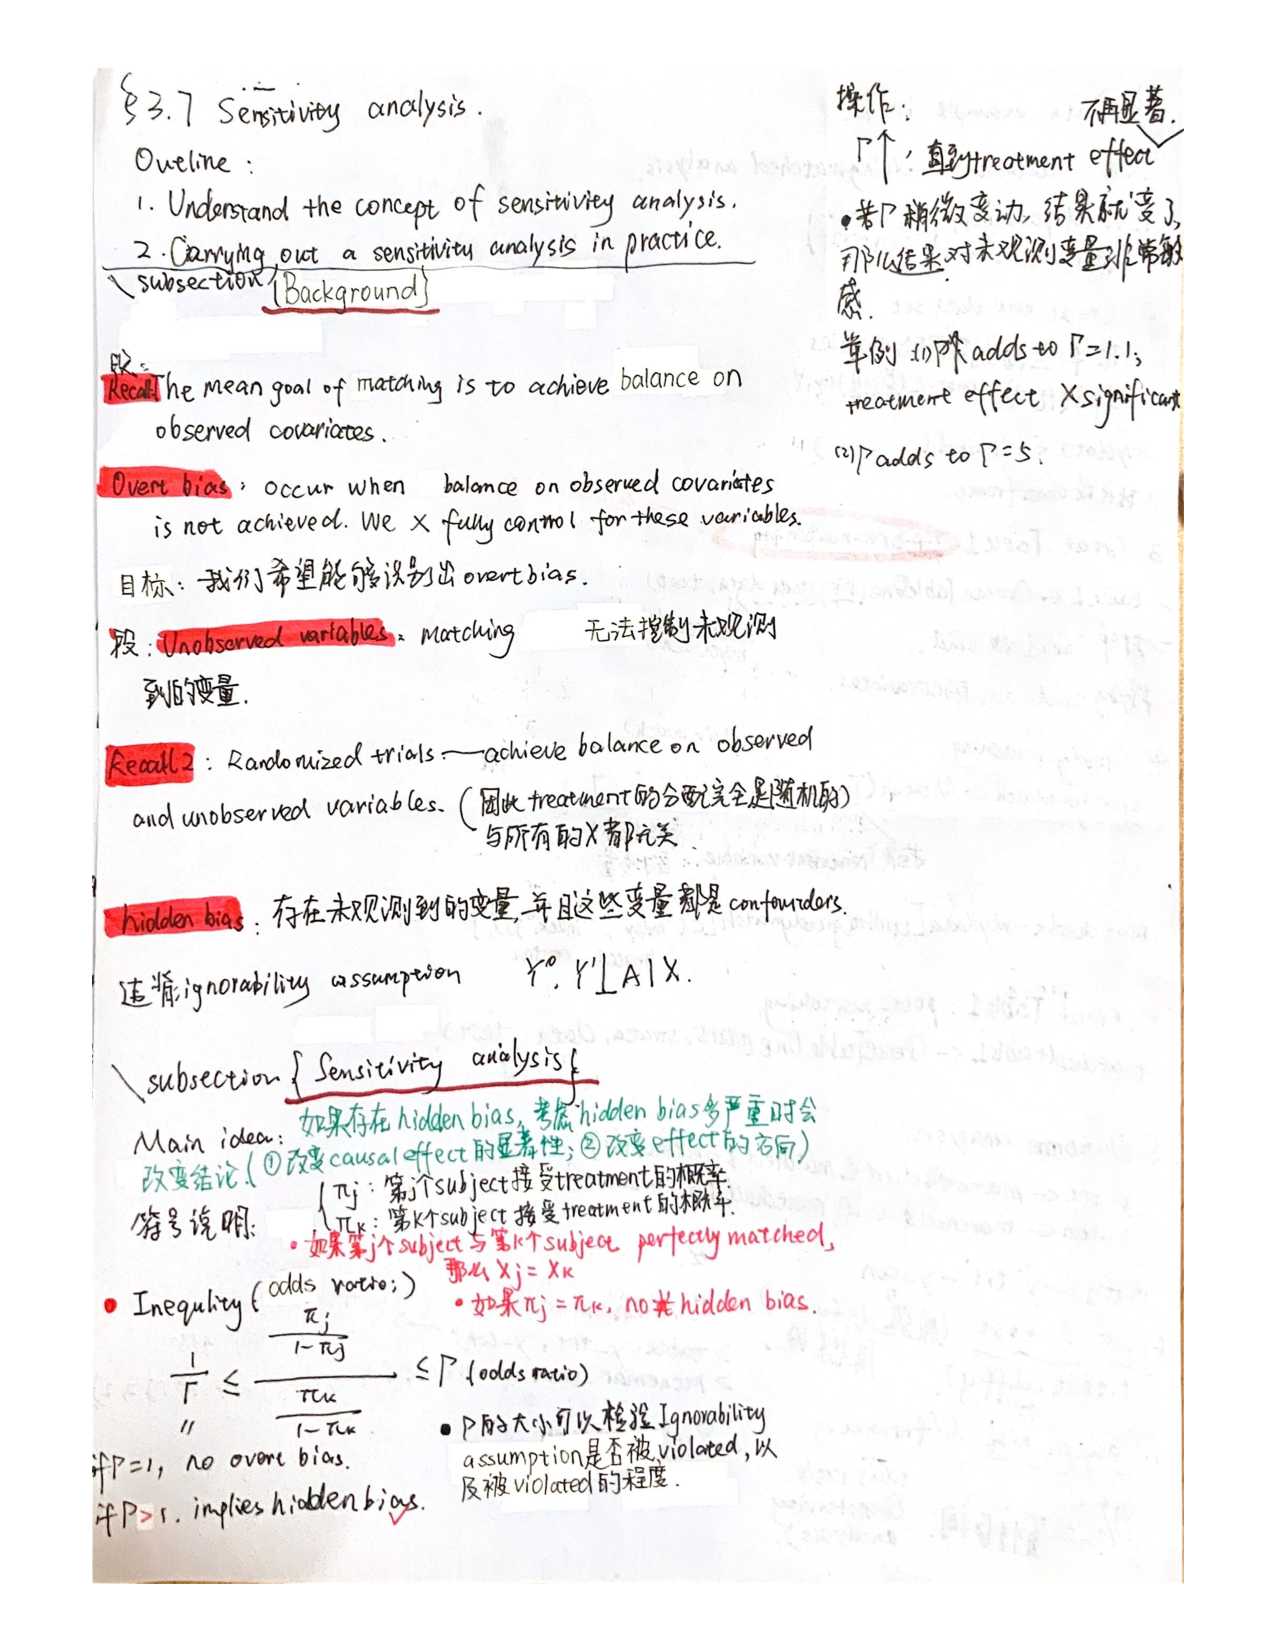
\includepdf[pages=-]{figure/sen.pdf}
\begin{figure}[htbp]
	\setlength{\abovecaptionskip}{0pt}     %调整图片标题与图距离
	\setlength{\belowcaptionskip}{10pt}
	\vspace{-0cm}  %调整图片与上文的垂直距离
	\setlength{\abovecaptionskip}{-0cm}   %调整图片标题与图距离
	\setlength{\belowcaptionskip}{-0cm}   %调整图片标题与下文距离
	\centering
	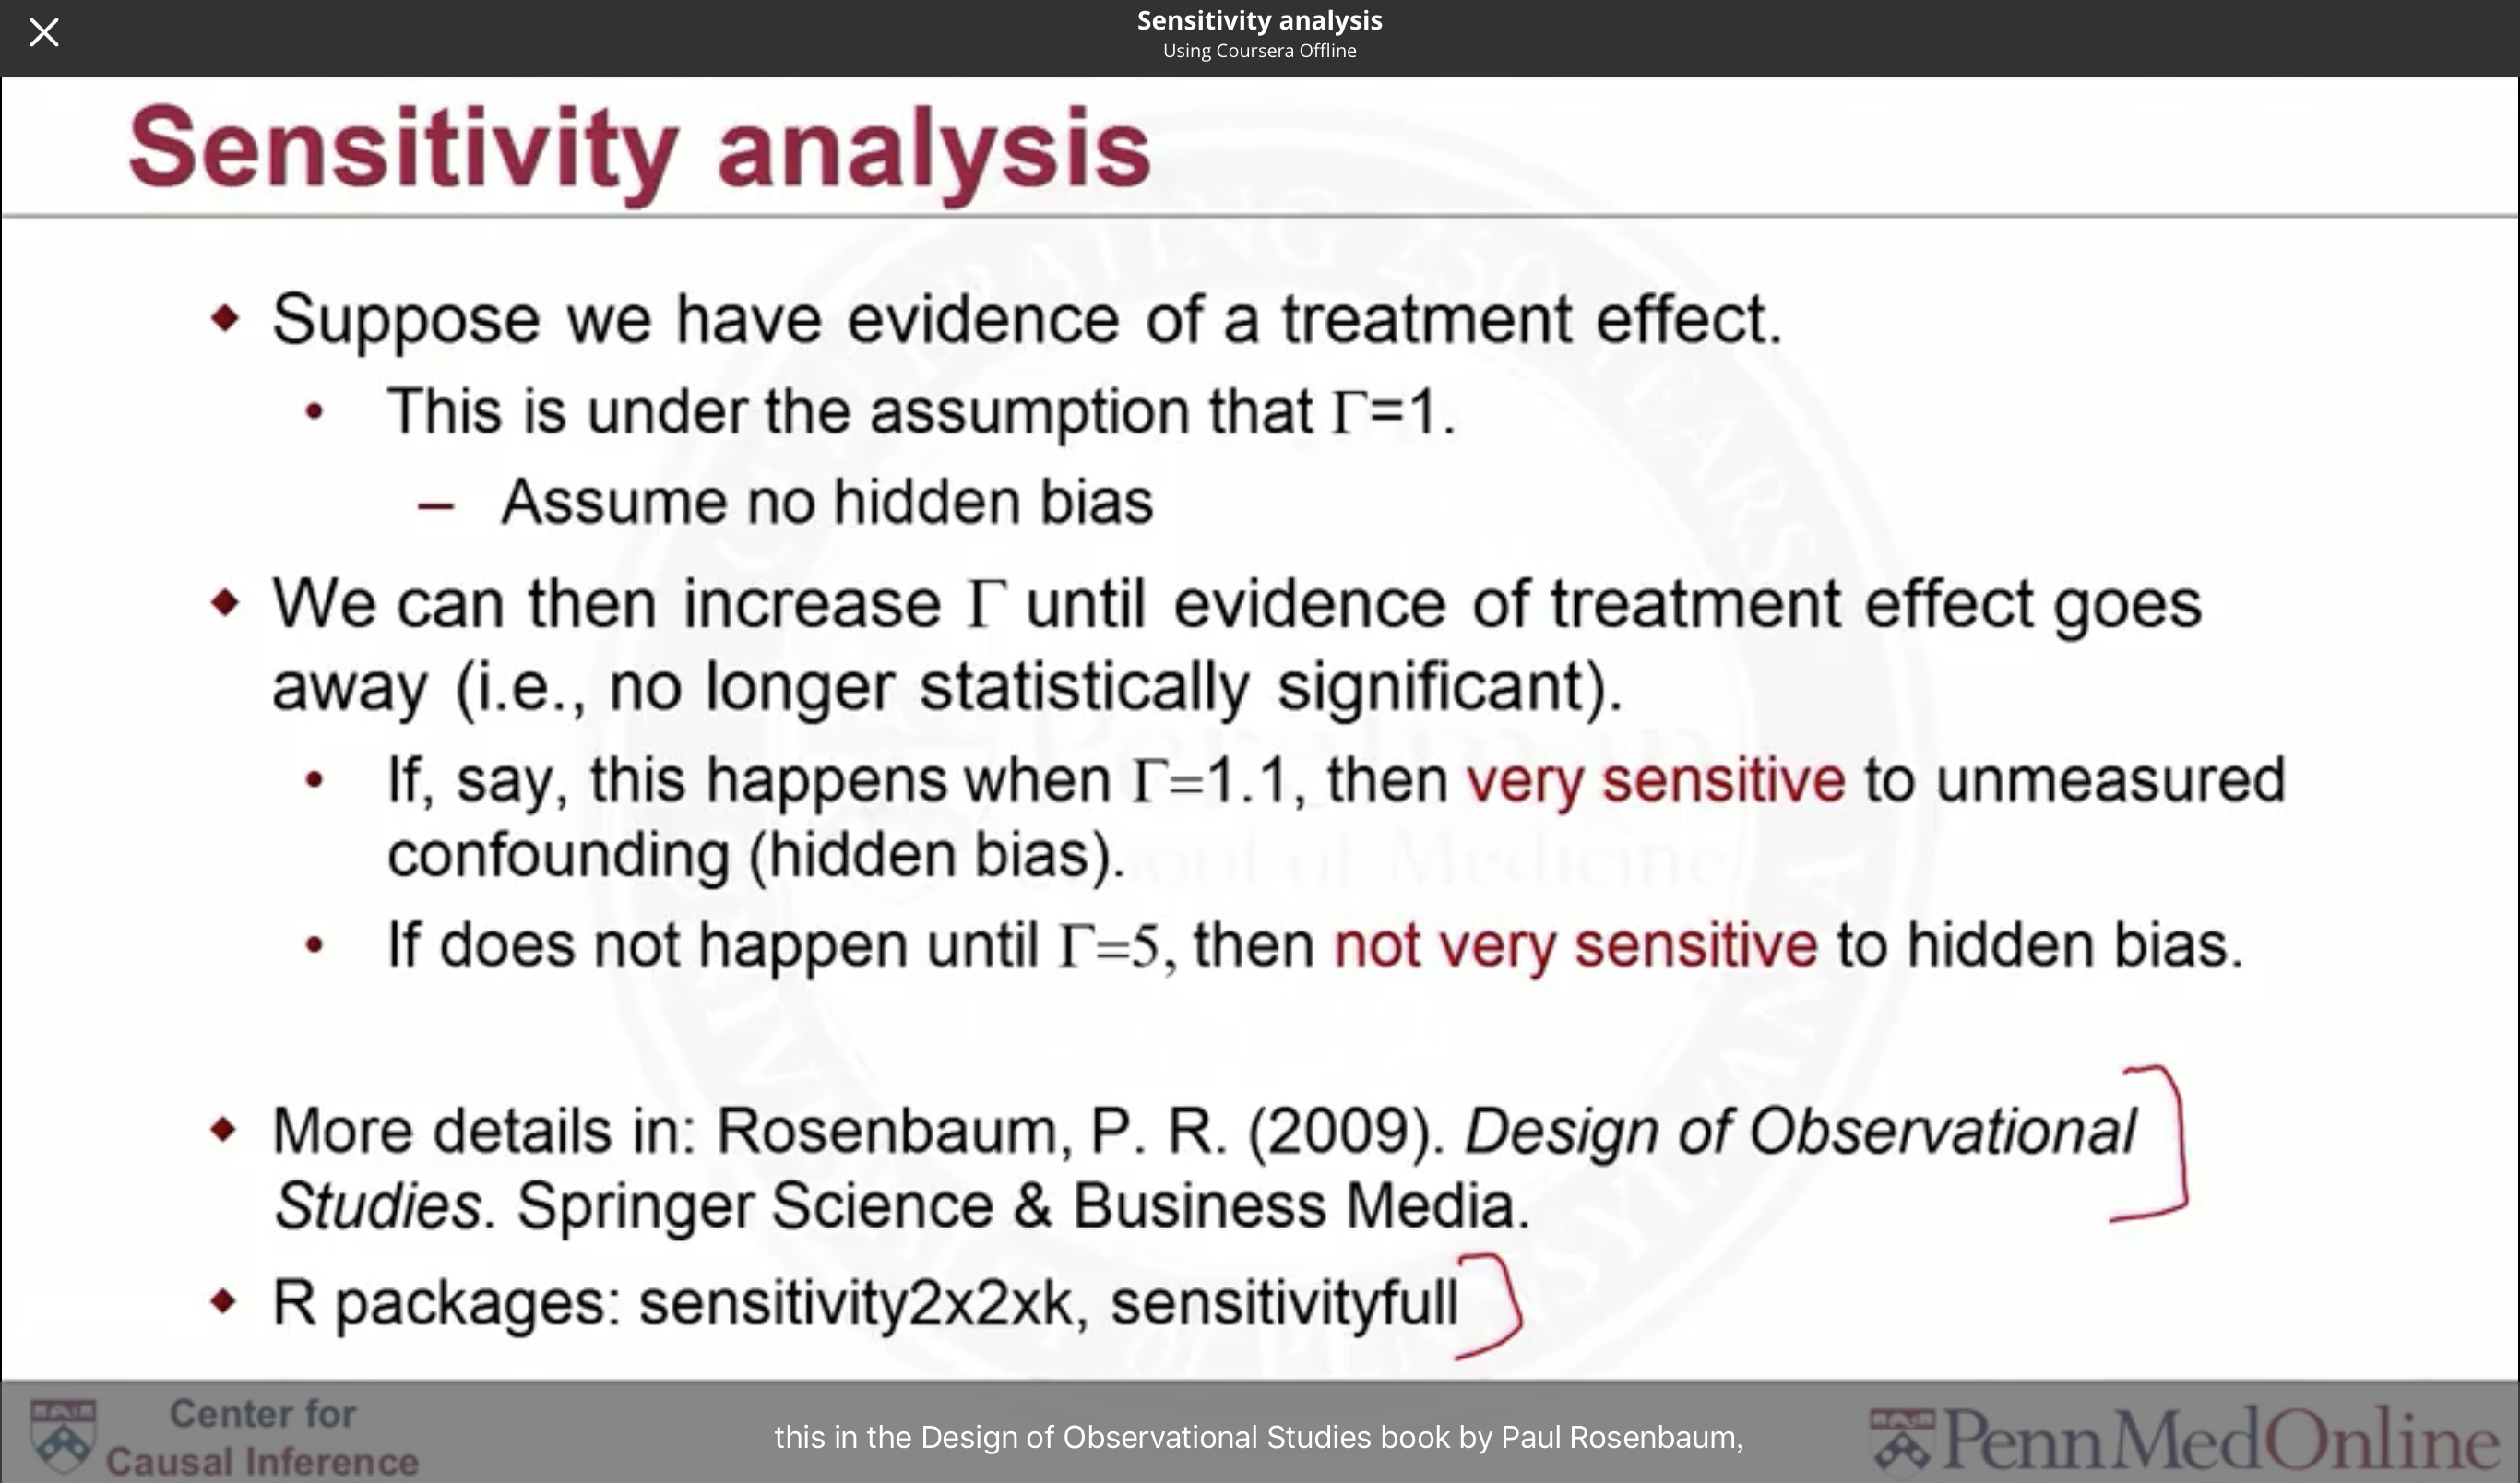
\includegraphics[width=0.8\textwidth]{figure/sensitivity.jpg}
	\caption{Sensitivity analysis}
	\label{sen}
\end{figure}

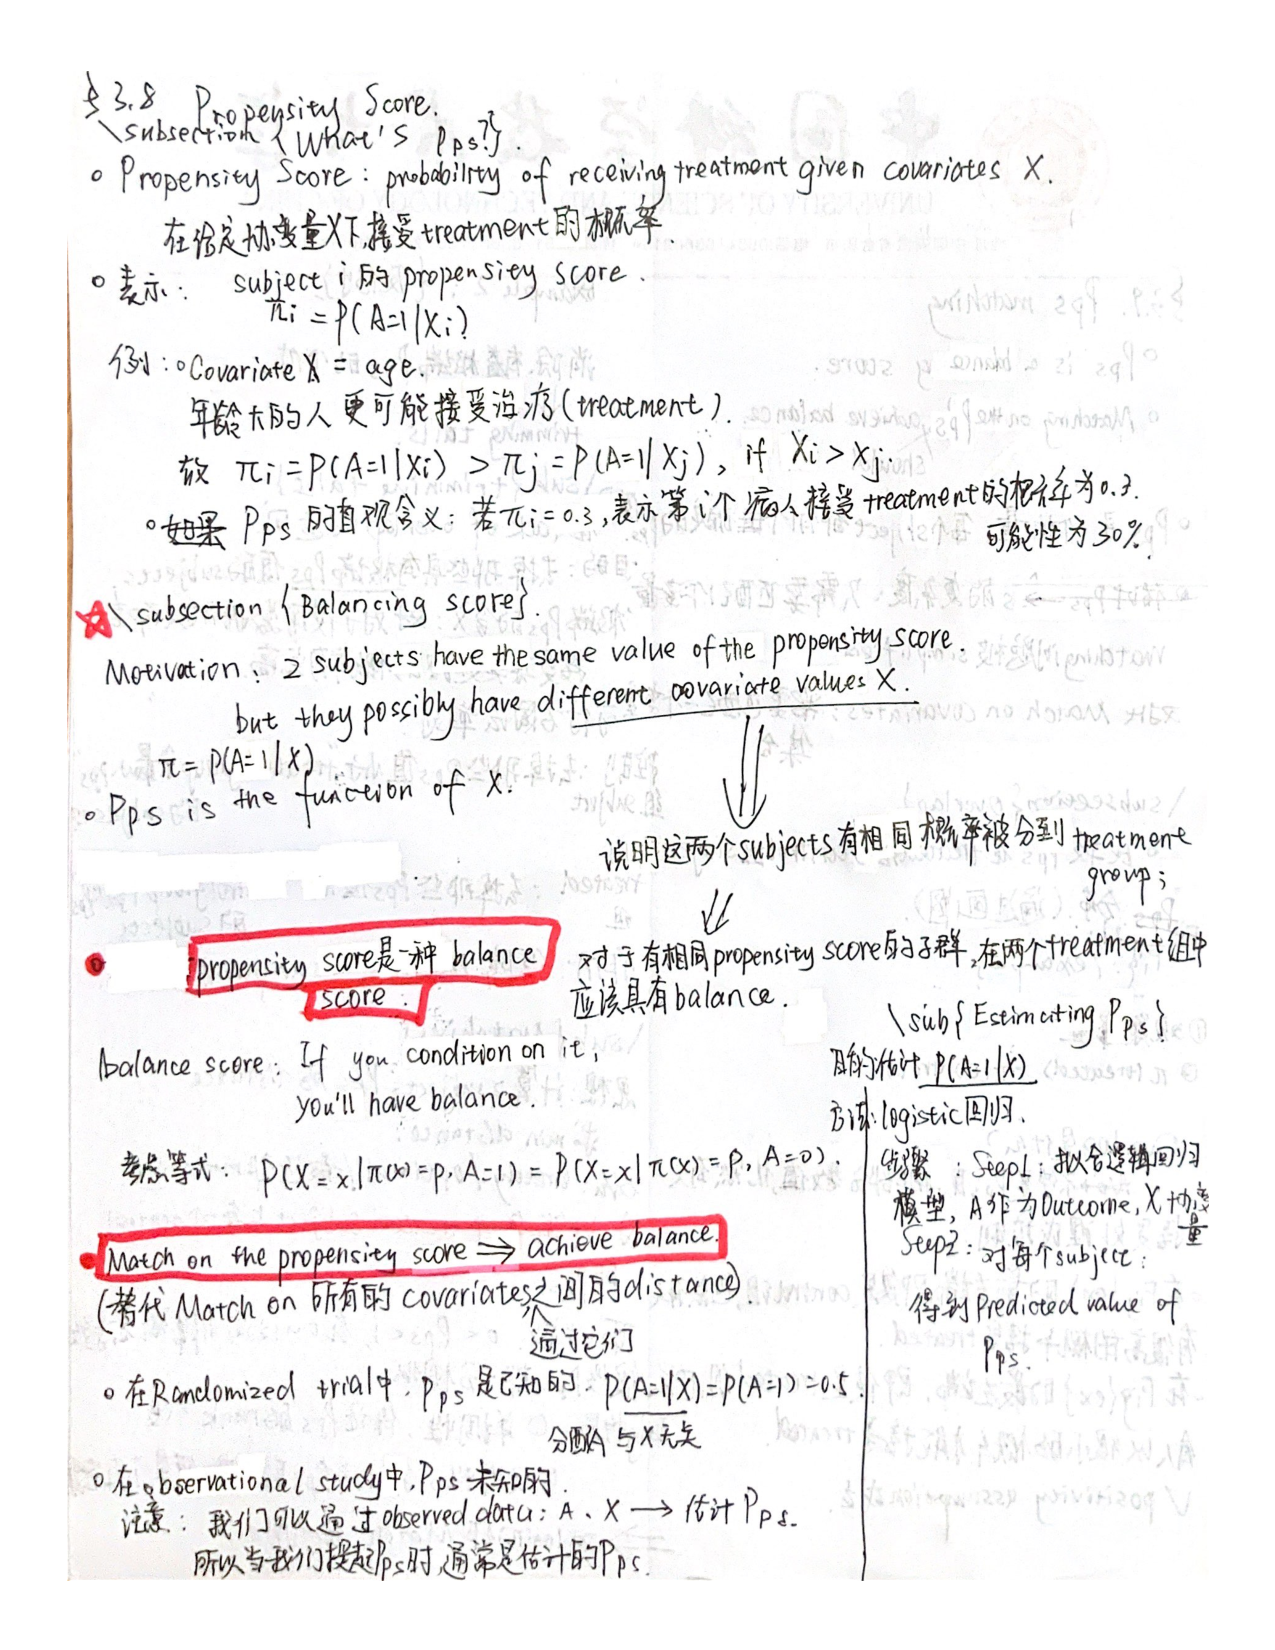
\includepdf[pages={1}]{figure/3pdf.pdf}
\includepdf[pages={2,3}]{figure/3pdf.pdf}

\begin{figure}[htbp]
	\setlength{\abovecaptionskip}{0pt}     %调整图片标题与图距离
	\setlength{\belowcaptionskip}{10pt}
	\vspace{-0cm}  %调整图片与上文的垂直距离
	\setlength{\abovecaptionskip}{-0cm}   %调整图片标题与图距离
	\setlength{\belowcaptionskip}{-0cm}   %调整图片标题与下文距离
	\centering
	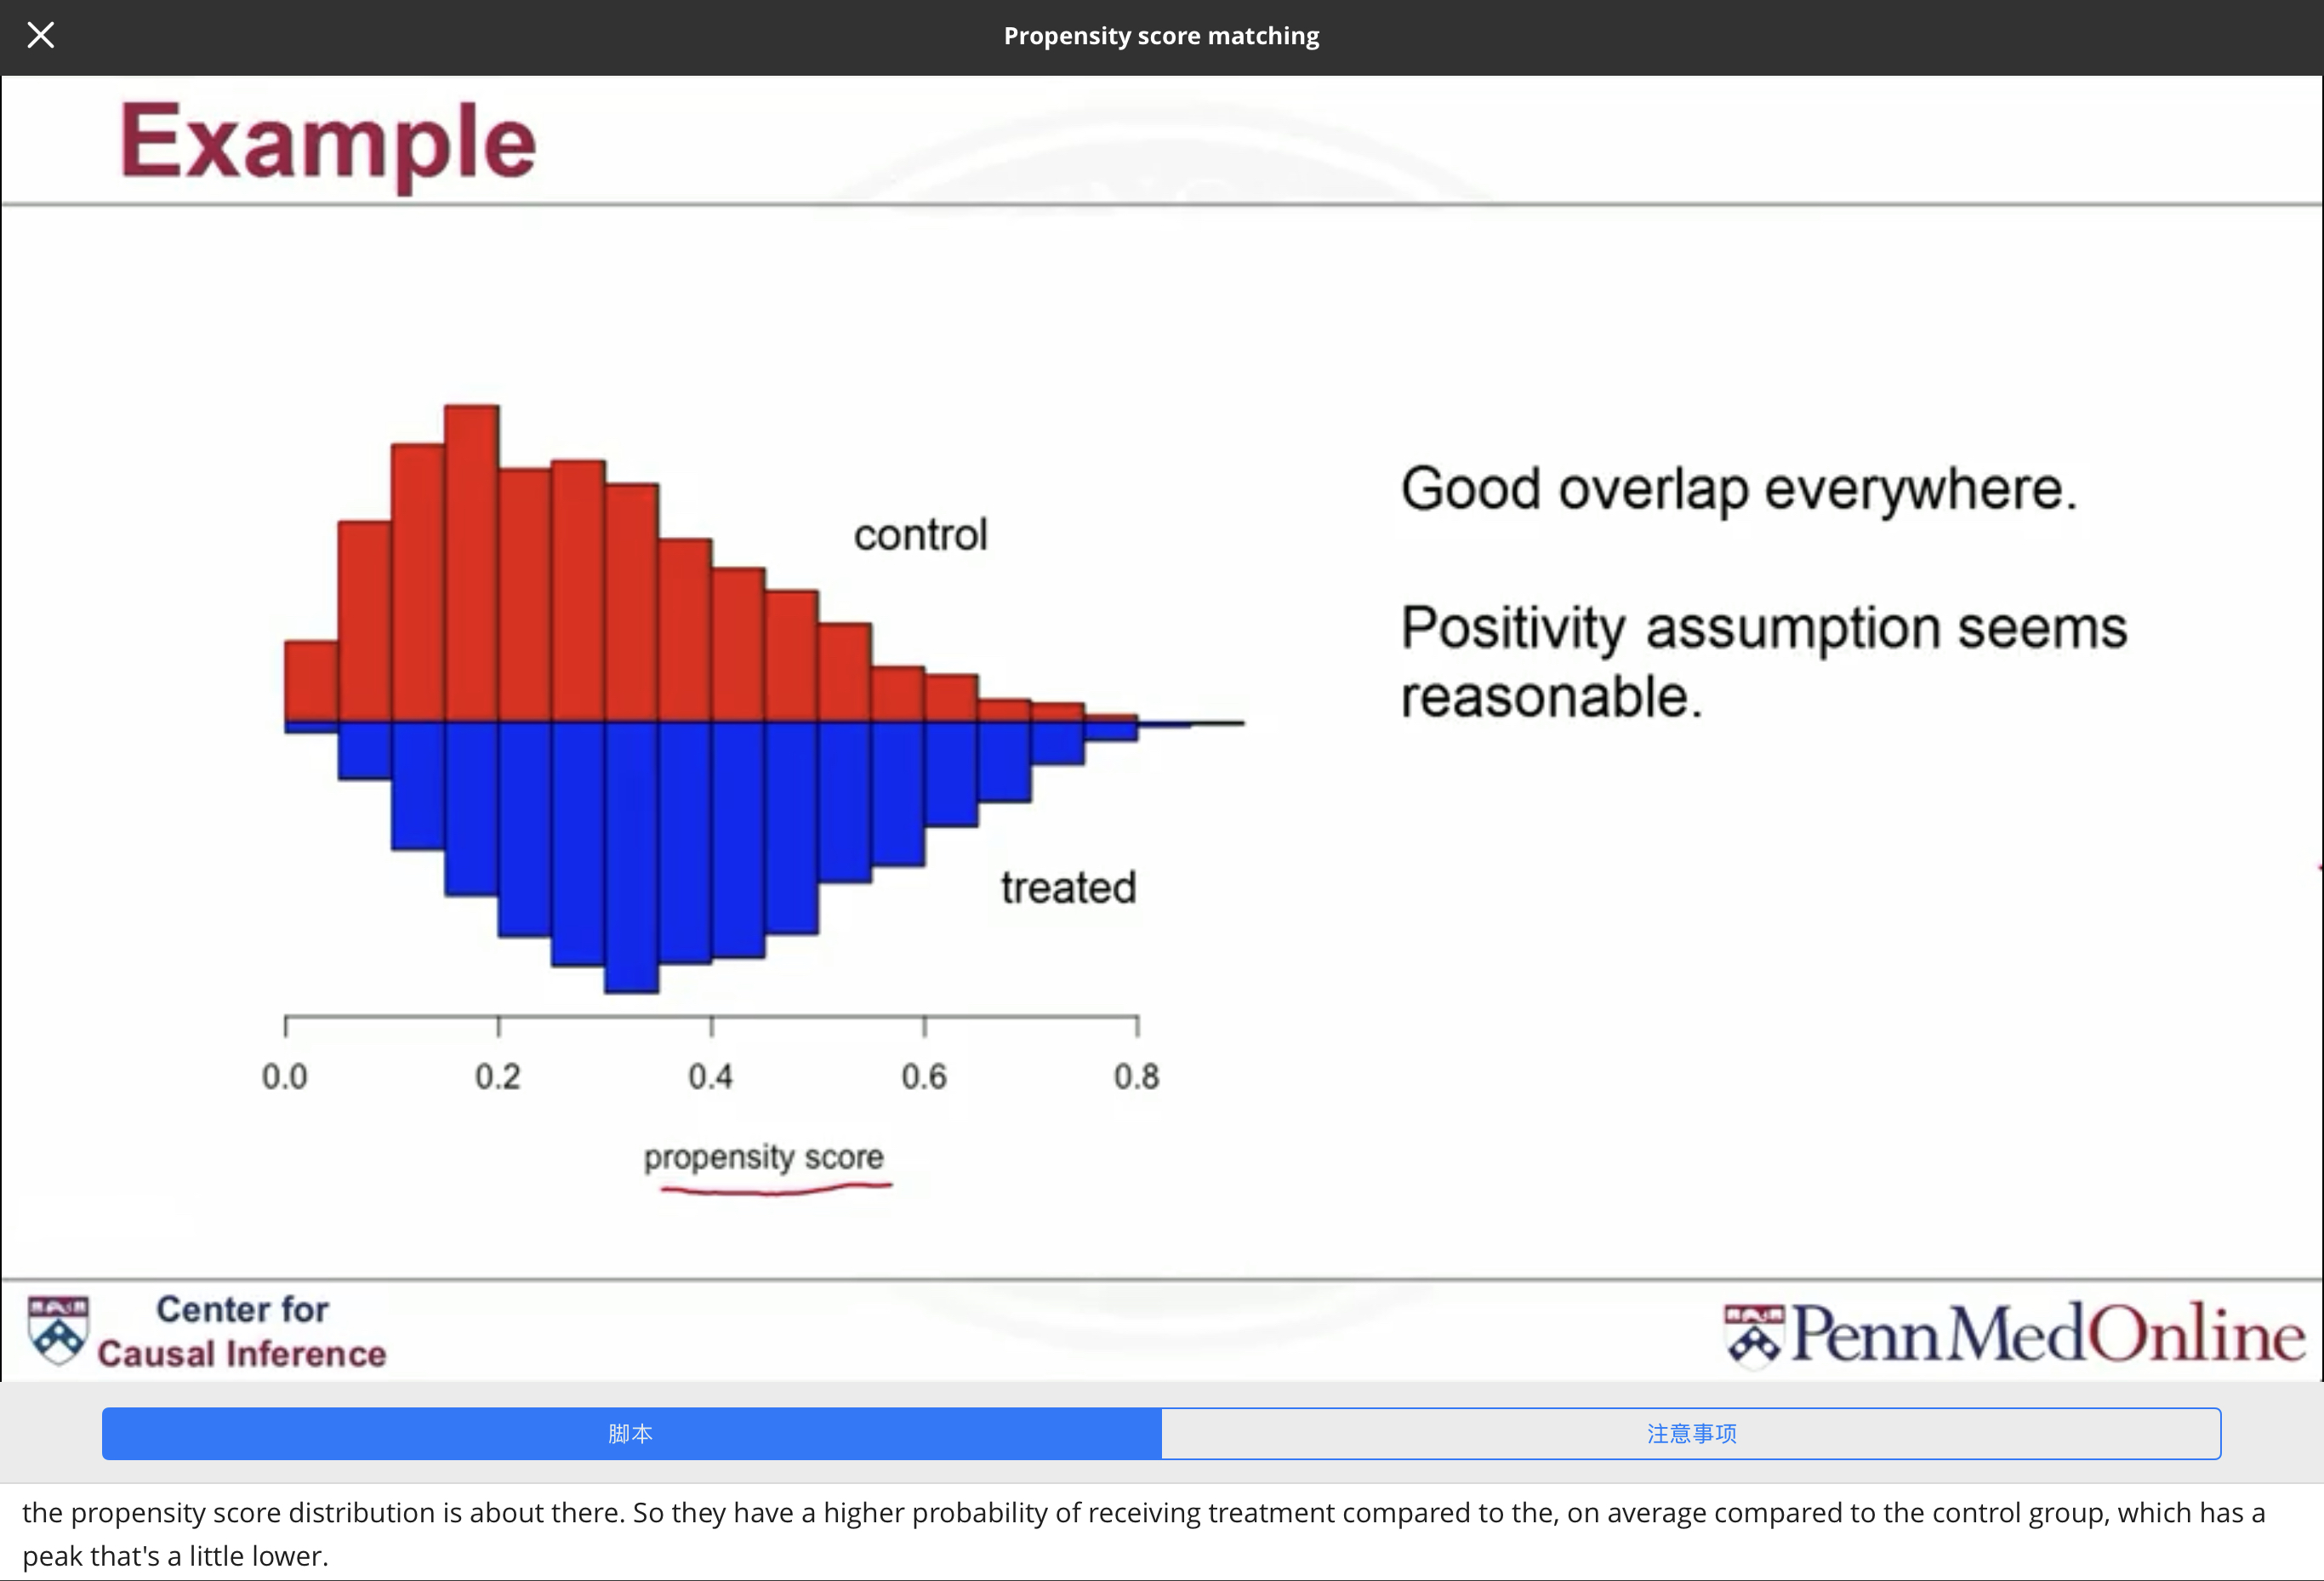
\includegraphics[width=0.8\textwidth]{figure/Example.jpg}
	\caption{Example}
	\label{Example}
\end{figure}
\begin{figure}[htbp]
	\setlength{\abovecaptionskip}{0pt}     %调整图片标题与图距离
	\setlength{\belowcaptionskip}{10pt}
	\vspace{-0cm}  %调整图片与上文的垂直距离
	\setlength{\abovecaptionskip}{-0cm}   %调整图片标题与图距离
	\setlength{\belowcaptionskip}{-0cm}   %调整图片标题与下文距离
	\centering
	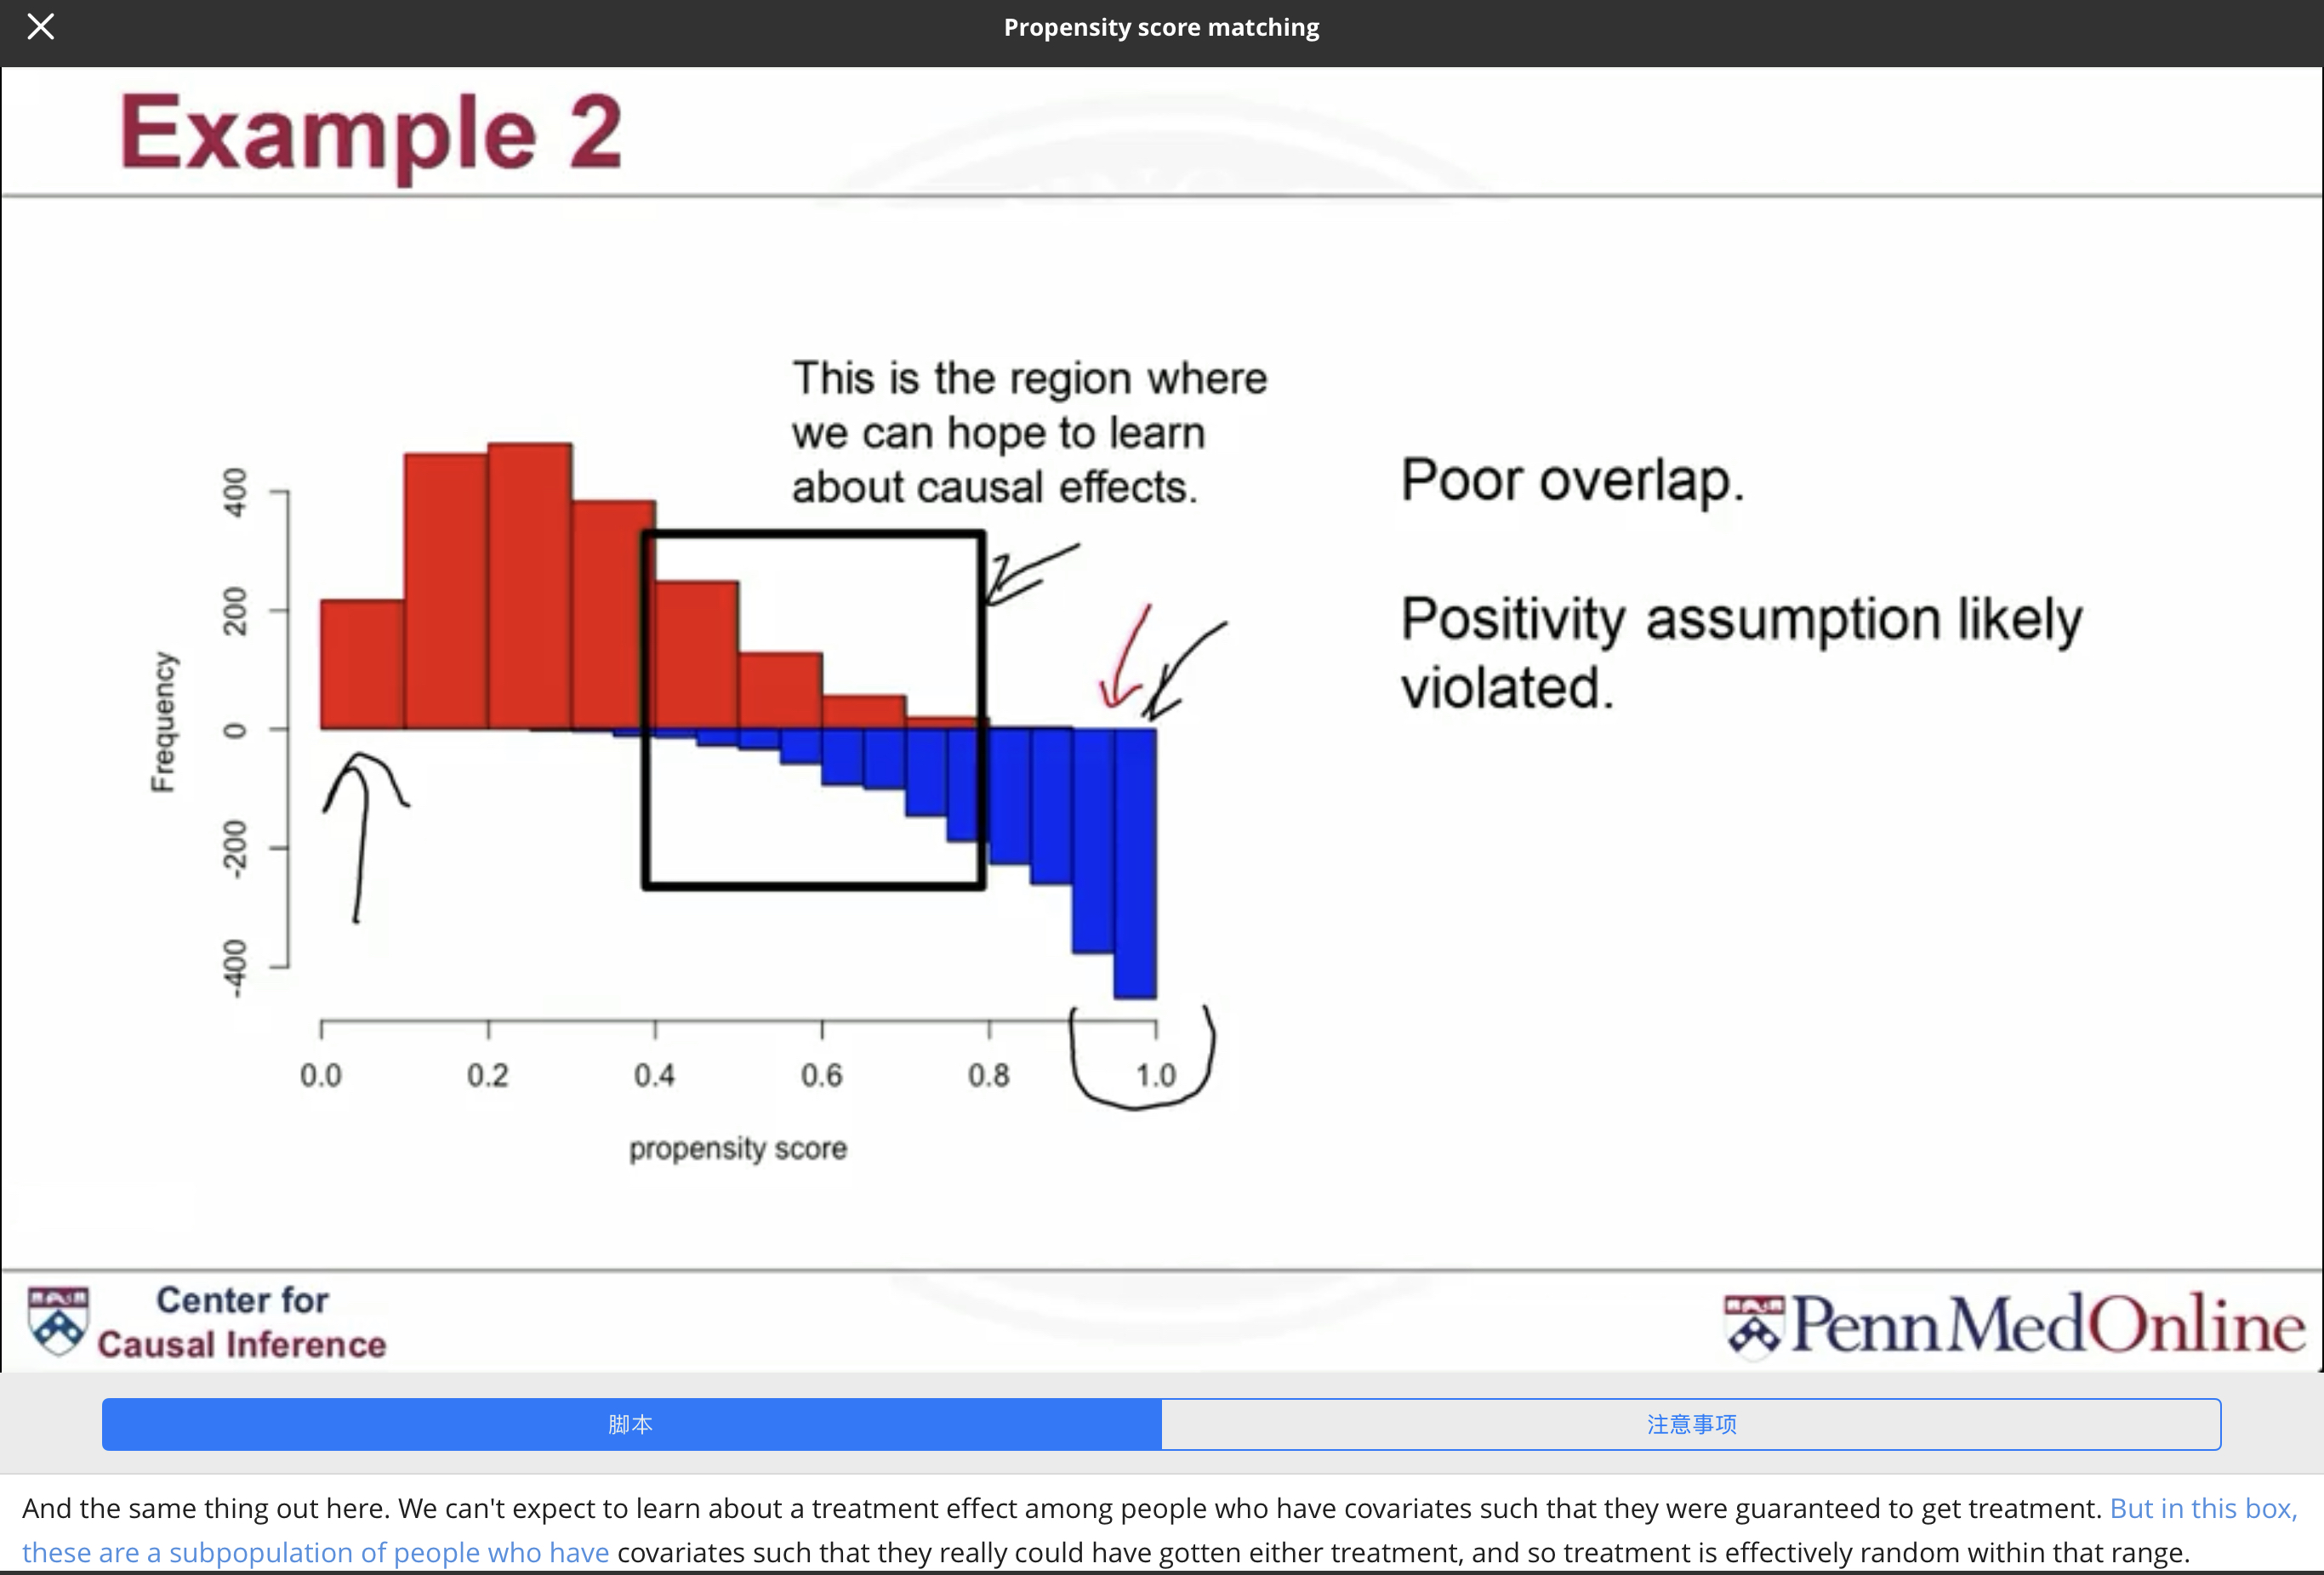
\includegraphics[width=0.8\textwidth]{figure/Example2.jpg}
	\caption{Example2}
	\label{Example2}
\end{figure}

\begin{figure}[htbp]
	\setlength{\abovecaptionskip}{0pt}     %调整图片标题与图距离
	\setlength{\belowcaptionskip}{10pt}
	\vspace{-0cm}  %调整图片与上文的垂直距离
	\setlength{\abovecaptionskip}{-0cm}   %调整图片标题与图距离
	\setlength{\belowcaptionskip}{-0cm}   %调整图片标题与下文距离
	\centering
	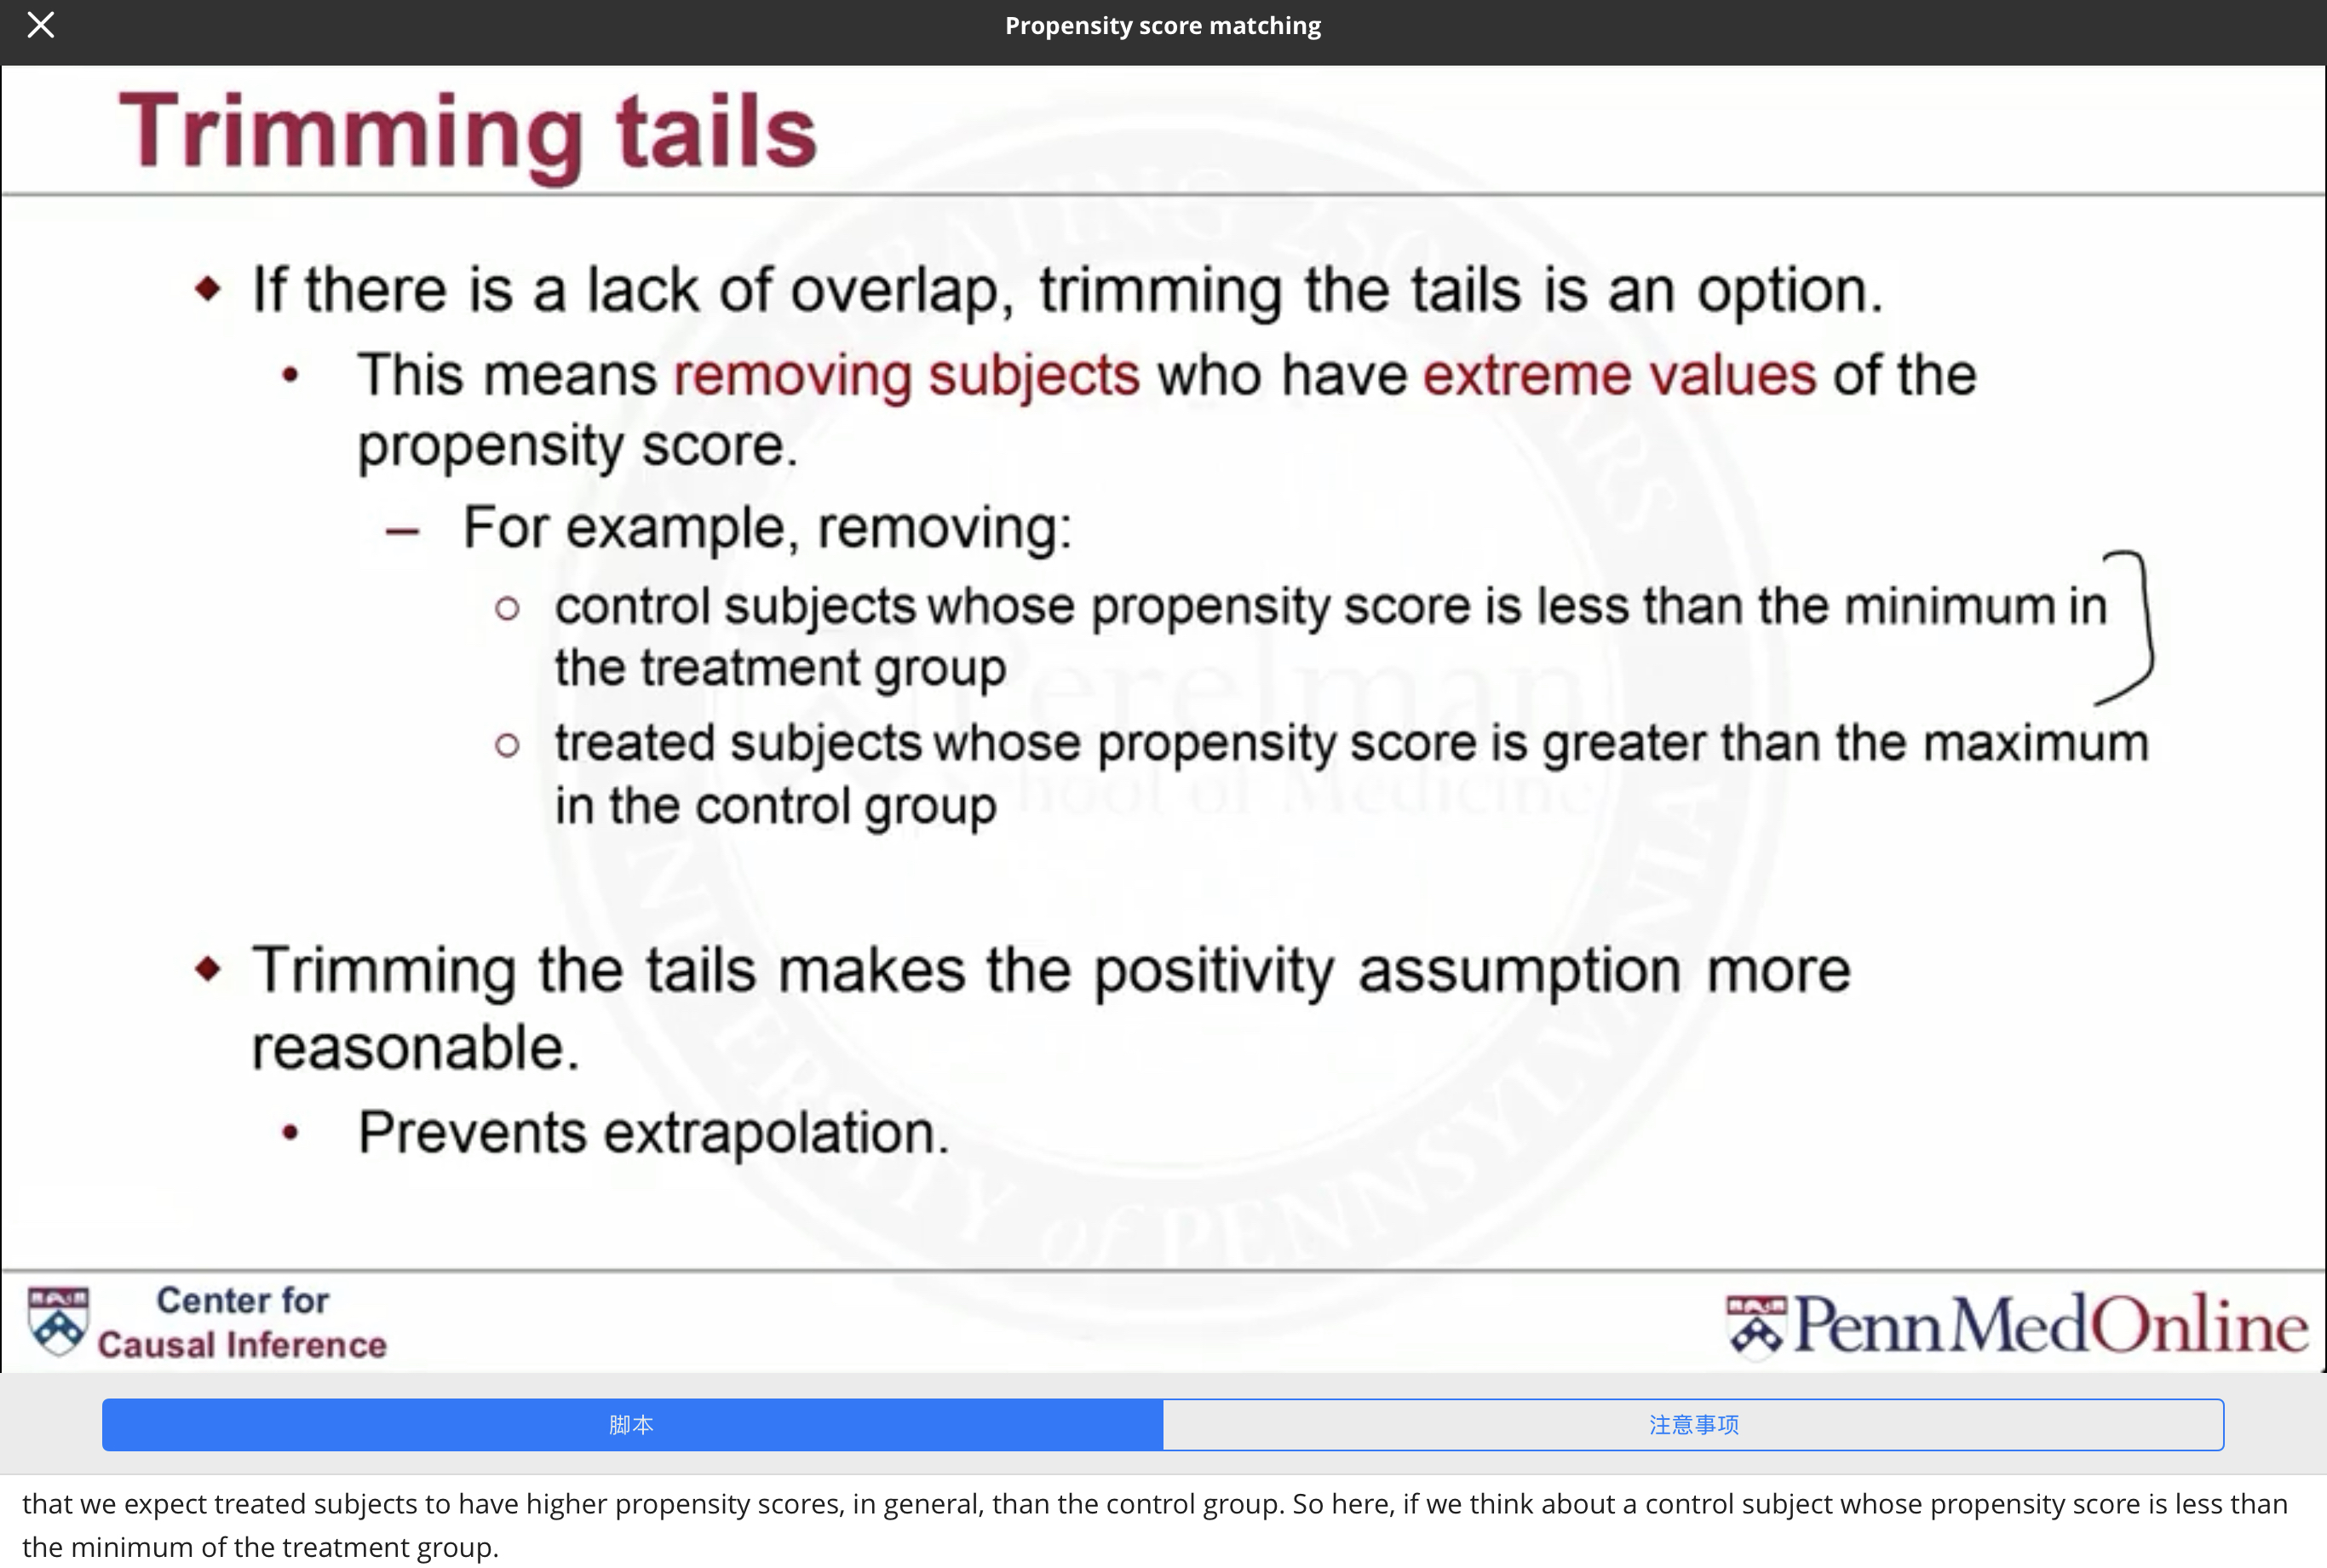
\includegraphics[width=0.8\textwidth]{figure/trim.jpg}
	\caption{Trimming tails}
	\label{trim}
\end{figure}

\begin{figure}[htbp]
	\setlength{\abovecaptionskip}{0pt}     %调整图片标题与图距离
	\setlength{\belowcaptionskip}{10pt}
	\vspace{-0cm}  %调整图片与上文的垂直距离
	\setlength{\abovecaptionskip}{-0cm}   %调整图片标题与图距离
	\setlength{\belowcaptionskip}{-0cm}   %调整图片标题与下文距离
	\centering
	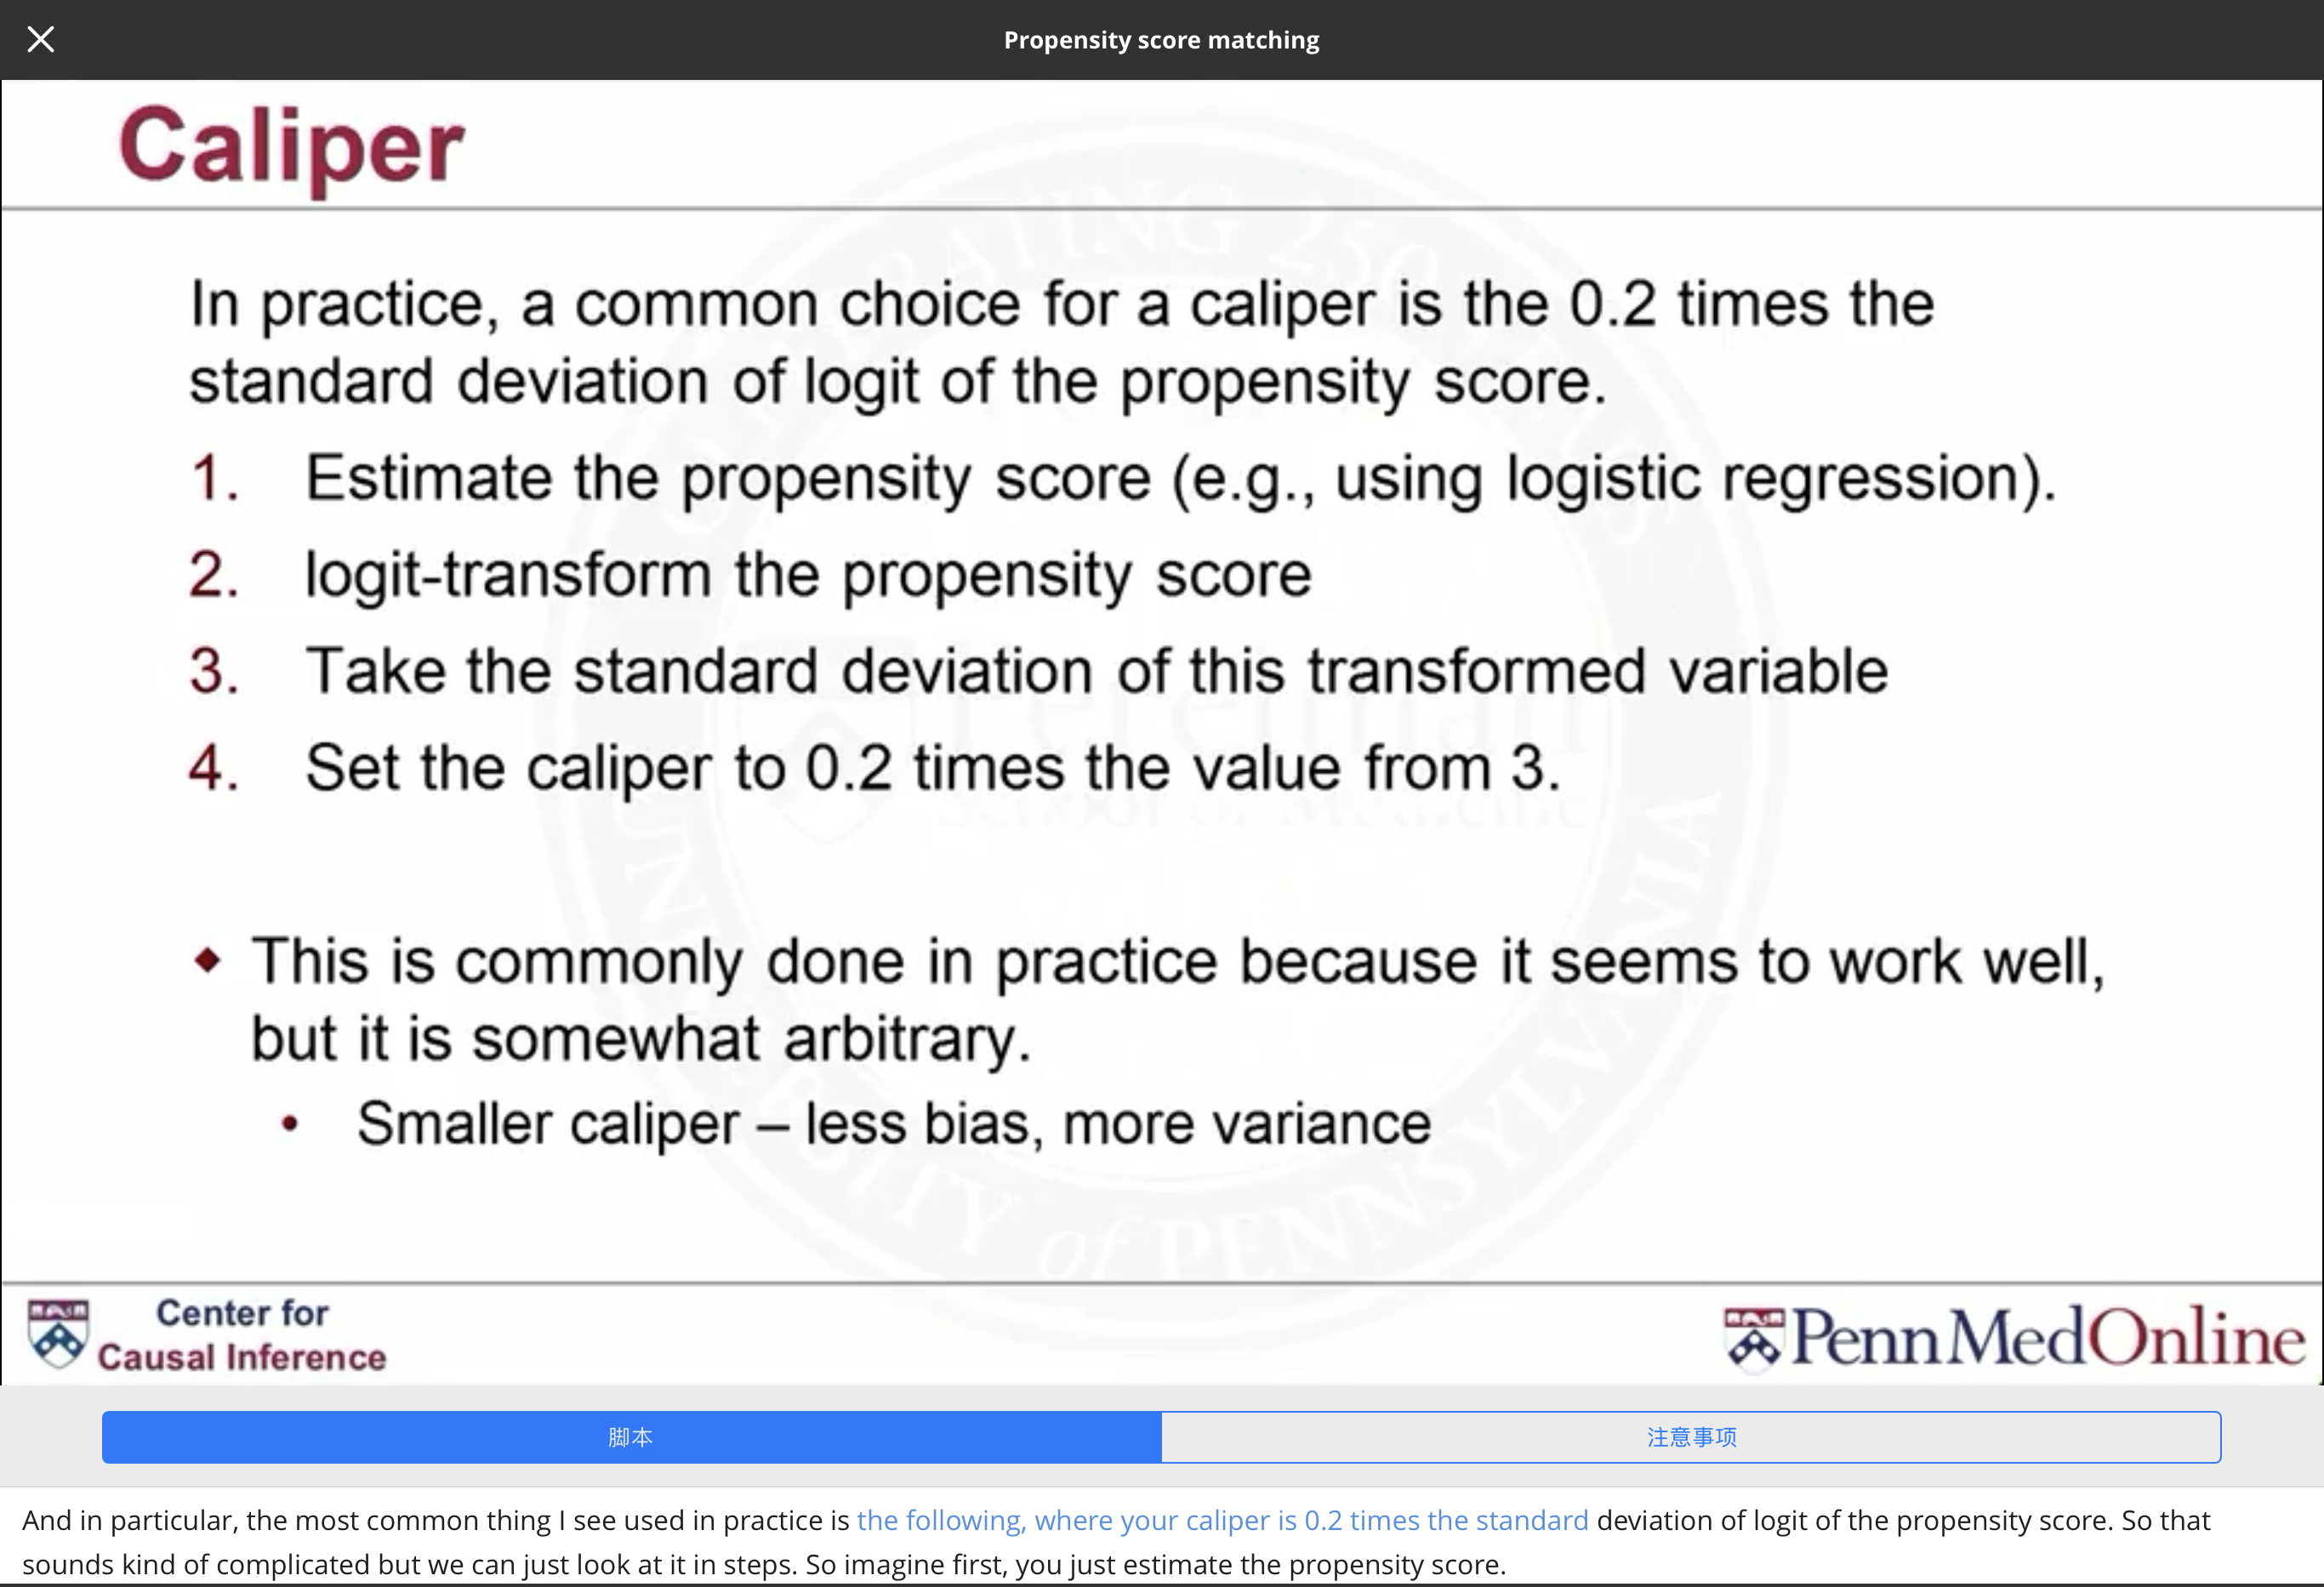
\includegraphics[width=0.8\textwidth]{figure/caliper.jpg}
	\caption{Caliper}
	\label{caliper}
\end{figure}


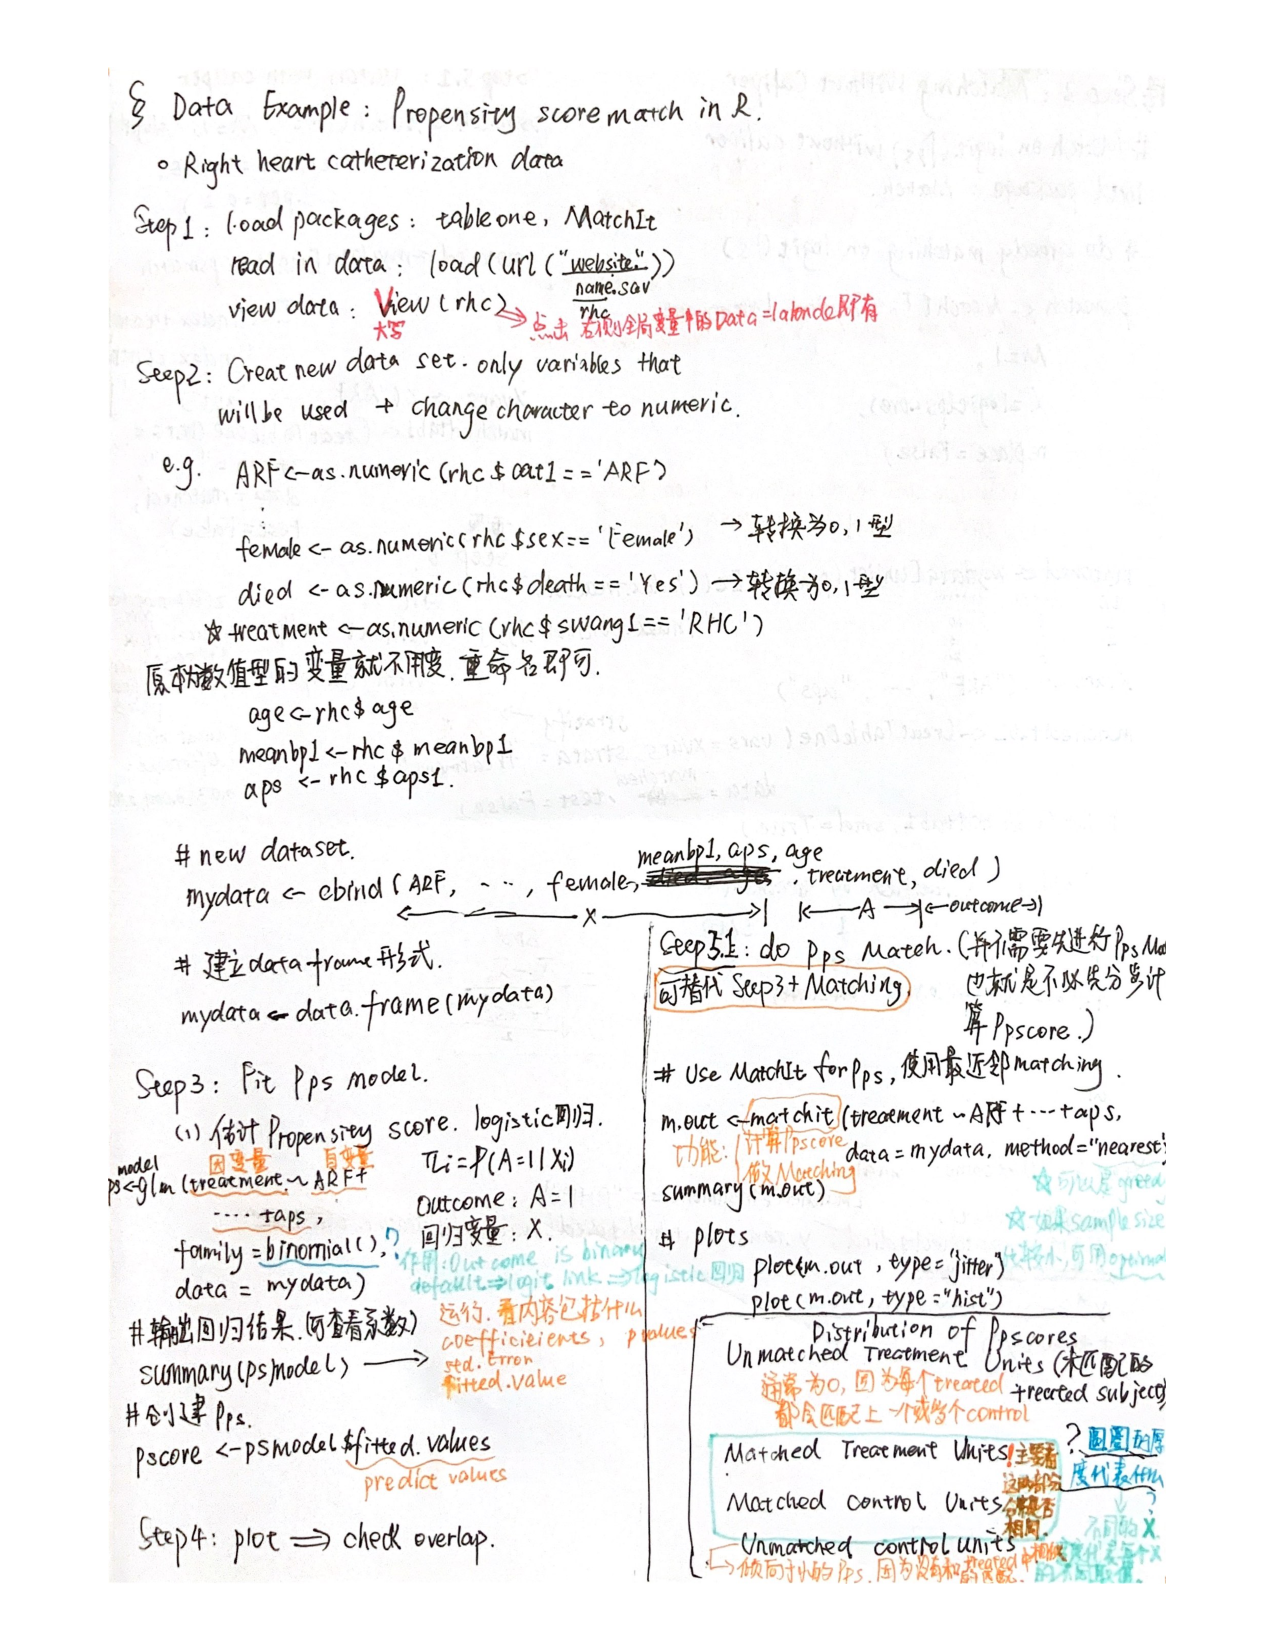
\includepdf[pages=-]{figure/psmatchinR.pdf}